\documentclass[12pt,lot, lof]{puthesis}
\newcommand{\proquestmode}{}


%%%%%%%%%%%%%%%%%%%%%%%%%%%%%%%%%%%%%%%%%%%%%%%%%%%%%%%%%%%%%\
%%%% Author & title page info

%%%%%%%%%%%%%%%%%%%%%%%%%%%%%%%%
\usepackage{color}
\usepackage{booktabs}

\usepackage{color}
\usepackage{url}
\usepackage{amsmath,amsthm,amssymb}
\usepackage{algorithm,algpseudocode}
\usepackage{enumerate}
\usepackage{multirow}
\usepackage{dirtytalk}
\usepackage{balance}
\usepackage{graphicx}
\usepackage{adjustbox}
\usepackage{enumitem}
\graphicspath{{/home/hrishi/work/thesis/pictures/}}


\title{ Comparative Analysis between Micro and Macro Agent Evacuation Using PedSim Simulator   }


\submitted{March 2019}  % degree conferral date (January, April, June, September, or November)
\copyrightyear{2019}  % year in which the copyright is secured by publication of the dissertation.
\author{Hrishikesh Narayanankutty}
\adviser{Professor Henry Muccini}  %replace with the full name of your adviser
%\departmentprefix{Program in}  % defaults to "Department of", but programs need to change this.
\department{Informatics}

%%%%%%%%%%%%%%%%%%%%%%%%%%%%%%%%%%%%%%%%%%%%%%%%%%%%%%%%%%%%%\
%%%% Tweak float placements
% From: http://mintaka.sdsu.edu/GF/bibliog/latex/floats.html "Controlling LaTeX Floats"
% and based on: http://www.tex.ac.uk/cgi-bin/texfaq2html?label=floats
% LaTeX defaults listed at: http://people.cs.uu.nl/piet/floats/node1.html

% Alter some LaTeX defaults for better treatment of figures:
    % See p.105 of "TeX Unbound" for suggested values.
    % See pp. 199-200 of Lamport's "LaTeX" book for details.
    %   General parameters, for ALL pages:
    \renewcommand{\topfraction}{0.85}	% max fraction of floats at top
    \renewcommand{\bottomfraction}{0.6}	% max fraction of floats at bottom
    %   Parameters for TEXT pages (not float pages):
    \setcounter{topnumber}{2}
    \setcounter{bottomnumber}{2}
    \setcounter{totalnumber}{4}     % 2 may work better
    \setcounter{dbltopnumber}{2}    % for 2-column pages
    \renewcommand{\dbltopfraction}{0.66}	% fit big float above 2-col. text
    \renewcommand{\textfraction}{0.15}	% allow minimal text w. figs
    %   Parameters for FLOAT pages (not text pages):
    \renewcommand{\floatpagefraction}{0.66}	% require fuller float pages
	% N.B.: floatpagefraction MUST be less than topfraction !!
    \renewcommand{\dblfloatpagefraction}{0.66}	% require fuller float pages

% The documentclass already sets parameters to make a high penalty for widows and orphans. 

%%%%%%%%%%%%%%%%%%%%%%%%%%%%%%%%%%%%%%%%%%%%%%%%%%%%%%%%%%%%%\
%%%% Use packages

%\usepackage{amsfonts}

%%% For figures
\usepackage{graphicx}
%\usepackage{subfig,rotate}

%%% for comments
\usepackage{verbatim}

%%% For tables
\usepackage{multirow}
% Longtable lets you have tables that span multiple pages.
\usepackage{longtable}

% Booktabs produces far nicer tables than the standard LaTeX tables.
%   see: http://en.wikibooks.org/wiki/LaTeX/Tables
\usepackage{booktabs}

%set parameters for longtable:
% default caption width is 4in for longtable, but wider for normal tables
\setlength{\LTcapwidth}{\textwidth}



%%%%%%%%%%%%%%%%%%%%%%%%%%%%%%%%%%%%%%%%%%%%%%%%%%%%%%%%%%
%%% Printed vs. online formatting
\ifdefined\printmode

% Printed copy
% url package understands urls (with proper line-breaks) without hyperlinking them
\usepackage{url}


\else

\ifdefined\proquestmode
%ProQuest copy -- http://www.princeton.edu/~mudd/thesis/Submissionguide.pdf

% ProQuest requires a double spaced version (set previously). They will take an electronic copy, so we want links in the pdf, but also copies may be printed or made into microfilm in black and white, so we want outlined links instead of colored links.
\usepackage{hyperref}
\hypersetup{bookmarksnumbered}

% copy the already-set title and author to use in the pdf properties
\makeatletter
\hypersetup{pdftitle=\@title,pdfauthor=\@author}
\makeatother

\else
% Online copy

% adds internal linked references, pdf bookmarks, etc

% turn all references and citations into hyperlinks:
%  -- not for printed copies
% -- automatically includes url package
% options:
%   colorlinks makes links by coloring the text instead of putting a rectangle around the text.
\usepackage{hyperref}
\hypersetup{colorlinks,bookmarksnumbered}

% copy the already-set title and author to use in the pdf properties
\makeatletter
\hypersetup{pdftitle=\@title,pdfauthor=\@author}
\makeatother

% make the page number rather than the text be the link for ToC entries
%\hypersetup{linktocpage}
\fi % proquest or online formatting
\fi % printed or online formatting


%%%%%%%%%%%%%%%%%%%%%%%%%%%%%%%%%%%%%%%%%%%%%%%%%%%%%%%%%%%%%\
%%%% Define commands

% Define any custom commands that you want to use.
% For example, highlight notes for future edits to the thesis
%\newcommand{\todo}[1]{\textbf{\emph{TODO:}#1}}


% create an environment that will indent text
% see: http://latex.computersci.org/Reference/ListEnvironments
% 	\raggedright makes them left aligned instead of justified
\newenvironment{indenttext}{
    \begin{list}{}{ \itemsep 0in \itemindent 0in
    \labelsep 0in \labelwidth 0in
    \listparindent 0in
    \topsep 0in \partopsep 0in \parskip 0in \parsep 0in
    \leftmargin 1em \rightmargin 0in
    \raggedright
    }
    \item
  }
  {\end{list}}

% another environment that's an indented list, with no spaces between items -- if we want multiple items/lines. Useful in tables. Use \item inside the environment.
% 	\raggedright makes them left aligned instead of justified
\newenvironment{indentlist}{
    \begin{list}{}{ \itemsep 0in \itemindent 0in
    \labelsep 0in \labelwidth 0in
    \listparindent 0in
    \topsep 0in \partopsep 0in \parskip 0in \parsep 0in
    \leftmargin 1em \rightmargin 0in
    \raggedright
    }

  }
  {\end{list}}



%%%%%%%%%%%%%%%%%%%%%%%%%%%%%%%%%%%%%%%%%%%%%%%%%%%%%%%%%%%%%\
%%%% Front-matter

% For early drafts, you may want to disable some of the frontmatter. Simply change this to "\ifodd 1" to do so.
\ifodd 0
% front-matter disabled while writing chapters
\renewcommand{\maketitlepage}{}
\renewcommand*{\makecopyrightpage}{}
\renewcommand*{\makeabstract}{}

% you can just skip the \acknowledgements and \dedication commands to leave out these sections.

\else


\abstract{
% Abstract can be any length, but should be max 350 words for a Dissertation for ProQuest's print indicies (150 words for a Master's Thesis) or it will be truncated for those uses.
Disaster management pertains to coping with disaster, relief and evacuation in the event of a catastrophe. It is of paramount importance as it pertains to the protection of lives and property during the time of calamity. To mitigate the damage of such incidents, simulations are performed in order to formulate an efficient and optimized exit strategy for the people who are struck by such unfortunate incidents and to evacuate them to a safe zone as quickly as possible. The simulation of an evacuation of the participating agents broadly falls under three categories - Macro Agent Simulation, Micro Agent Simulation and/or a combination of Macro-Micro Agent Simulation (grouping according to age, gender, social ties such as family, friendships etc.). Although extensive work has been carried out to simulate disaster scenarios comprising of a massive number of agents with an aggregate set of characteristics (Macro Agent Simulation), very little work has been done so far to simulate realistic social behaviour of agents during a disaster scenario, especially pertaining to micro agent simulations. Realistic human and social behaviour characteristics are possible only through micro agent-based simulations as complex psychological and sociological paradigms can be mapped and hence dynamic real-time strategy decisions can be better understood, especially during a crisis. Through this thesis, I aim to present the simulation and comparison of various micro and macro agent scenarios.

In order to run the aforementioned simulations, an open source microscopic pedestrian simulator - PedSim is used. This tool not only simulates the various complex scenarios. it also provides visual feedback in real time. PedSim is a crowd simulation library capable of analysis of real time pedestrian flow rate. This agent-based model (ABM) tool is a class of computational models for simulating the actions and interactions of autonomous agents (either individual or collective entities such as organizations or groups) with a view to assessing their effects on the system as a whole. It combines elements of game theory, complex systems, emergency, computational sociology, multi-agent systems, and evolutionary programming. Although there are many proposed agent modelling simulators that are available, many if not most are with commercial license and do not support real time data flow. This tool is also customized and further extended in order to take an optimized routing algorithm for agents. The PedSim simulator is modelled for both indoor and outdoor areas (parking lots, forests etc.). The simulation tool is able to take sensory based data and apply them to the modelling agents/nodes to simulate real/design time analysis. The main advantage of this library is the architecture that enables visibility of users live using tcp/stream-based output through batch processing. The implementation is pure in C++ with minimal external dependencies like Qt Framework. The output of PedSim can be translated using a graphics engine to provide visually appealing realistic render of a walking person. The code is modular, scalable and open source available under GPL license. 

The main goal of this thesis is to exhibit an objective performance analysis and a comparison between an existing macro agent simulation algorithm against an optimized algorithm coupled with realistic constraints, testing them against a massively populated macro and micro agent model for real-time dynamic evacuation.
}

\acknowledgements{
%I would like to thank...
I would like to thank the Informatics department for providing all the support and guidance.I would like to thank my parents, without whom my life would not be possible. I would also like to thank my advisor, my dissertation committee, and my research collaborators because every graduate student needs to do so. And finally, I thank the members of the research group, for providing me so many opportunities to learn and grow. 

I finally thank the Amrita University and University of L'Aquila for selecting me for the I2Cost Dual Degree program that has catapulted me thus far and is continuing to do so. 
}

\dedication{To my parents and my dear brother, \newline I am grateful for your undying love and support through the challenges I face. I am the person I am today because of you. I shall always cherish your wisdom and presence in my life.}

\fi  % disable frontmatter


%%%%%%%%%%%%%%%%%%%%%%%%%%%%%%%%%%%%%%%%%%%%%%%%%%%%%%%%%%%%%\
%%%% Hide some chapters

%%% If you want to produce a pdf that includes only certain chapters, specify them with includeonly, in addition to including all chapters below.
%\includeonly{ch-intro/chapter-intro}
%%% You can also specify multiple chapters.
%\includeonly{ch-intro/chapter-intro,ch-usage/chapter-usage}
%\includeonly{chap1,chap2,chap3}


%%%%%%%%%%%%%%%%%%%%%%%%%%%%%%%%%%%%%%%%%%%%%%%%%%%%%%%%%%%%%
%%%% Notes:

% Footnotes should be placed after punctuation.\footnote{place here.}
% Generally, place citations before the period~\cite{anotherauthor}.
% The proper usage for i.e., and e.g., include commas ``(e.g., option A, option B)''

%%%%%%%%%%%%%%%%%%%%%%%%%%%%%%%%%%%%%%%%%%%%%%%%%%%%%%%%%%%%%
%%%% Import chapters

\begin{document}

\makefrontmatter


% If you've disabled frontmatter, you can insert the toc manually
%\tableofcontents\clearpage

% \include lets us split up the document (and each include starts a new page):

\chapter{Introduction\label{ch:intro}}

Due to increasing topological changes in urban environment, the human civilization has been subjected to increasing risk of disasters due to natural or artificial, and/or a combination of the two causes, since the better part of the modern era. Hence it has become an ever increasing need to design infrastructure to handle such disasters in the event it may occur. But even more so, the safe evacuation of people and personnel with the premises of the affected infrastructure takes precedence when dealing the necessary mitigation and disaster risk management. The evacuation time of people from a scene of disaster is extremely crucial in the case of an emergency in disaster situation. In order to reduce the time taken for evacuation, better and more robust exit strategy evacuation algorithms are developed which are used to model participating agents for their exit patterns and exit strategies and clock them based on performance, efficiency and practicality. In order to evaluate such parameters, evacuation simulation models have been developed and constantly tested over the years to investigate the emergency egress capabilities of the built environment for a variety of reasons including: difficulty in conducting real evacuation tests (drills); aiding building design and confirming conformity to building regulations; and even determining optimal evacuation routes for the building occupiers [1]. Computational models were first introduced in the early 1980s since the inception of computers. During the 90s, academic researchers aimed to improve these the capabilities of these models in order to optimize and improve the pathfinding performance of the evacuees and their corresponding movements [2]. Over the course of many years, these algorithms have become the industry standard to perform exit evacuation time and performance analysis. The purpose of this thesis is to study the state of the art algorithm and to draw comparisons between micro model agent simulation with respect to its counterpart, the macro model agent simulation.

\section{Motivation}
\label{sec:intro:Motivation}

Realistic simulations involve complex relationships between an individual and the surroundings. Three types of interactions are possible whilst the individual performs complex decision making during an evacuation scenario. Through this thesis I aim to optimize these three types of interactions through various constraints and real time elements. The following encounters may be classified as below \cite{ref1}:

\begin{itemize}
  \item People-people interactions -  interactions between participating evacuees.
  \item People-structure interactions- interactions within the enclosed topology.
  \item People- environment interactions- interactions with quarantined atmosphere (fire, smoke etc.) and possible debris. 
\end{itemize}

During disaster scenarios standard evacuation pathways are often rigid and cannot autonomously provide modification for an exit strategy as the disaster ensues. The evacuees often find themselves in situations that force them to rely on general guidelines about how to react in emergency evacuation \cite{ref3}.  While such dynamic hazards cannot all be dealt with, using the traditional approach, Lujak, M., Billhardt H., Dunkel, J. et al \cite{ref4} attempts to help the evacuees adapt to the changing topography of the environment due to hazard dynamics by updating a real time monitoring system using an IoT architecture built in place within the premises of the said topology of the building. The above mentioned work uses a combination of IoT devices to sense and identify and provide real-time monitoring for the participating agents. Our work also obtains data from real time sources and then it is simulated with both macro and micro based agent models and then used to analyse and draw conclusions from the resulting data.

\section{Agent Based Model Simulation}
\label{sec:intro:Agent Based Model Simulation}

The present thesis is a design of a computational software using Agent Based Model (ABMS) to help speedy evacuation in emergency situations. Our software architecture help optimise the navigational flow rate in cases of real-time disaster management. The scenario is that of many victims are struck up in a very large building in the event of an occurrence of a disaster like fire, earthquake, poisonous chemical gas leakage, imminent bomb attack, potential imminent building collapse (similar to that of twin towers of 9/11). As a side benefit the experience acquired gives valuable information in the case of architecture design at the time of building construction itself. By conveying a suggestive path for each individual in the building at the time of disaster, the panic, erratic and groping movements are reduced to minimum helping to achieve a streamlined flow. Bottlenecks in the flow are avoided by redirecting people to alternate paths. The benefit of the overall perspective of the scenario and informed management is instantaneously conveyed to each and every individual in real time. The floor capacities and width of the doors and passageways form part of the constraints in the modelling. This is scalable and generic version.

\section{PedSim Simulator}
\label{sec:intro:PedSim Simulator}

PedSim is a pedestrian simulator tool designed as a front end to facilitate disaster management scenarios. Disaster management plans are multi-layered and topology specific. Tools catering to disaster management require the users to input topographic information and also provide crowd/agent location information. This aggregate of data is then processed initially to create a layout of the premises. The layout defines several rules and boundary conditions imposing restrictions for the crowd to navigate. Such information can be used to instantly model very specific scenarios such as evacuation of specific floors of a building. Since, PedSim enables input of design specific topology, protocols can be established quickly for speedy evacuation. The second part includes behaviour analysis of crowd during different disaster patterns. The social behaviour of victims in disaster afflicted scenarios have been of keen interest to researchers over the recent years. Disaster affected regions often portray victims who exhibit severe trauma or stress leading to emotional/psychological shut down or present themselves making erratic decisions etc. This tool enables a platform for crowd flow modelling. Erratic movement patterns can be modelled, simulated and visualized to study the impact and speed of evacuation. Such processed information can be used to provide instructions or navigation guidelines for optimal evacuation. PedSim also allows for real time monitoring of crowds providing instant feedback on the visual front end. This enables redirection of crowds for balancing congestion while developing exit strategies. Each exit can also be associated with restrictive exit capacity and corresponding flow rate ensuring crowd balancing.  The architectural design of the tool itself takes into account various factors such as streaming and batch processing of time critical data within permissible thresholds.

\section{Objectives and Approach}
\label{sec:intro:Objectives and Approach}

My work pertains to application of PedSim on our university building to implement and analyze the impacts of crowd evacuation during a disaster. The university building taken into consideration for our present study is level 3 of building (Coppito 0). The area under consideration is divided into 18 blocks. Each block consists of a set number of cells. Each cell represents a cubicle or a room. There are 26 cubicles/rooms in all. There is also one conference hall and two generic multipurpose areas used for allied purposes. In addition, there are several hallways and pathways for navigation. This area has four key exits distributed across the different boundary walls of the premises. At any given time, each cell hosts atmost twenty agents, reaching a maximum during peak hours of 10am to 2 pm Italy time. The premises often on average hosts about 100 people. We architected pedestrian flow simulations during a generic disaster which can include earthquake, fire and chemical leakage. The data is used to generate crowd clusters during events other than disasters such as workshops, cafeteria gatherings, conference gatherings etc. The figure \ref{clutter} shows a typical population cluster during a conference gathering. 

This thesis presents a case study where the Coppito 0 building is simulated during a disaster scenario using grid geometry based navigation algorithm as presented in the “An IoT Software Architecture for an Evacuable Building Architecture” by H.Muccini et.al \cite{ref5}. 

\begin{figure}[H]
  \centering
  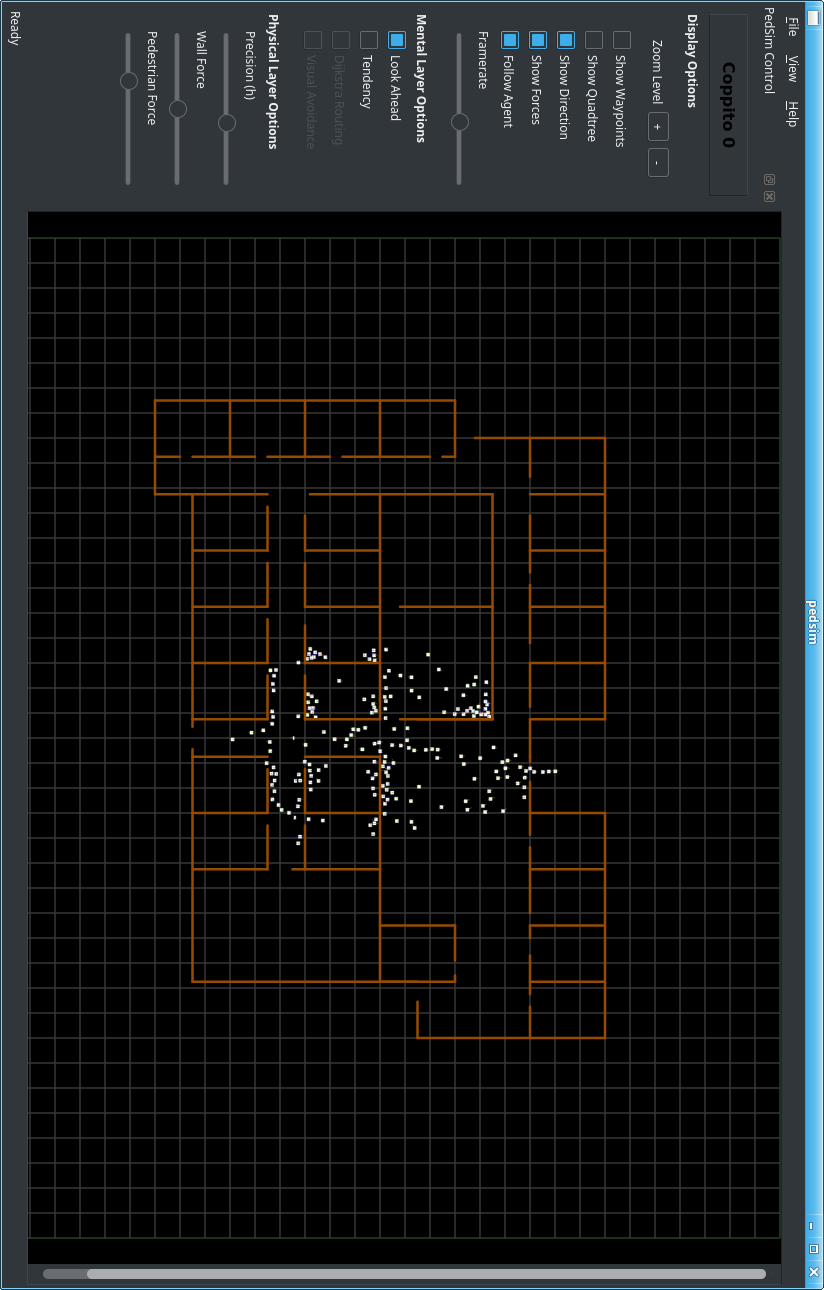
\includegraphics[scale=0.6]{implementation/clutter.png}
	\caption{Agent Cluster Formation in Coppito 0 Building}
  \label{clutter}
\end{figure}

The work also involves in expanding the capabilities of the existing PedSim simulation tool to include the new topology and the also to incorporate the algorithm and also further extended developed from the aforementioned paper and perform a real time analysis between micro and macro agents with the following criteria:

\begin{itemize}
  \item specifying the cells by social distances
  \item respecting the area capacity and doors capacities constraints
  \item setting the speed accordingly for various groups
  \item simulating social attachment among some agents 
\end{itemize}

As it is evident from the above constraints, the goal of this algorithm and this simulation is to make exit strategies as realistic as possible. By grouping certain agents together for instance, we can achieve realistic movement of participating agents, as in reality, people usually move in groups. families, friends etc. Furthermore, congestion is a big part of the evacuation scenario, as it is congestion that determines how fast or efficient the evacuation of agents occur and also how it would take to move groups of people. With groups of people clumped together, the next most natural constraint would be to assign varying speeds as not all agents and not all groups of agents travel with the same speed across the topology of the building. There is also one other constraint which determines the cell capacity, which determines how spaced out and occupied agents are in a room, a hall or a passageway. This also help determine how many can get through a single doorway in order to transition from one passageway to another. This of course leads to previously mentioned issue of congestion. 

All these constraints are hence taken into account as the simulation is performed in order to clock and test for the performance time and efficiency of the algorithm used for micro and macro model simulation.

\section{Thesis Outline}
\label{sec:intro:Thesis Outline}

The structure of the thesis is formulated as follows: chapter 2 provides a detailed literature and background work pertaining to the area of agent based simulation models and exit strategies. Chapter 3 focuses on the implementation details of the algorithm and specific scenario details that are incorporated in order to extend the algorithm in order to adapt it to a more realistic setting and also technical details regarding the PedSim simulation environment. Chapter 4 presents the results of the comparisons of the optimized(realistic) algorithm between the macro and micro agent simulation setting and to chart out the various performance metrics that are obtained. Chapter 5 attempts to draw conclusions based on the obtained performance metrics and also present the future work related to the aforementioned. This thesis also provides a technical appendix for reference for the simulation of various micro and macro agent scenarios within the environment of PedSim.

\chapter{Related Work\label{ch:pastwork}}

In this section the background literature and the work related to agent based simulation is dicussed. 

% include other files for sections of this chapter. These use the 'input' command since each section within a chapter should not start a new page.
% If you want to swap the order of sections, it is as simple as reversing the order you include them. 
\section{Pre-Modern Disaster Preparedness, Management and Relief Techniques}
\label{sec:pastwork:Pre-Modern Disaster Preparedness, Management and Relief Techniques}

Although disasters have existed throughout the history of the universe for all living organisms, human beings are perhaps the only one to be affected on a massive scale as a collective group as we are vulnerable and weak compared to other animals that live and co-exist with us. Hence human beings have taken many steps over the years fortifying and defending ourselves as best as we can through the various buildings and escape routes we design. The early inhabitants of mankind were not idle and did not become easy victims. There is historical evidence that the early man took various measures in order to cope with, reduce and mitigate risks. The mere fact that they chose to inhabit caves are a testament to this theory \cite{ref6}.

The ancient man also used other natural techniques for disaster preparedness. One of the prominent ones include the observation of animals since they are very perceptive to natural disasters, animal behavior can and has been used for the better part of the millenia to predict the onset of a natural disaster such as floods, earthquakes etc. One of the earliest works to be done in this field involves in the observation of the behavior of fish, specifically the catfish, as they were found to exhibit a definitive behavior in advance of the occurence of an earthquake \cite{ref7}. Other experiments and observations pertaining to such natural responses include the obeservation of ground electric field effects on behavior of Albino rats, Mongolian gerbils (sand rats), hair-footed Djungarian hamsters, guinea pigs, and red sparrows \cite{ref8}. A summary of such animal behavior and work is presented by Neeti Bhargava et. al. \cite{ref9}.

To combat various natural disasters that affect us, mankind has tried for over a millenia to improve and adapt buildings, and entire cities to cope during the time of a catatrosphe. There are two broad categories to the mitigation of these disasters that have been long employed \cite{ref10}:

\begin{itemize}
  \item structural based mitigation
  \item non-structural based mitigation
\end{itemize} 

Since my work pertains to indoor simulation and evacuation management, the discussion for non-structural mitigation forms here is considered unnecessary and beyond the scope of this thesis. Structural mitigation involves the presence of a building or a man-made mechanical or technological adaptations performed to reduce hazards and mitigate risks. The following sub-section expands more on the more modern techniques that have been developed over the course of the modern era and their implications. Although better and state of the art systems have been developed over the years, these systems have complications of their own. Failure of the perfect working of an evacuation system leads to the possible death of all the agents who are in need of evacuation. 

\section{Routing Algorithms and IoT Based Evacuation Management}
\label{sec:pastwork:Routing Algorithms and IoT Based Evacuation Management}

Routing algorithms and maze solving algorithms have especially been applied to the structural domains for the real time analysis of shortest paths and obstacle avoidance by both machine and human agents since the time the earliest shortest paths algorithms were developed. The development of the shortest path algorithm by Dijkstra in 1956, especially has seen a plethora of applications in various fields. As one can guess most of its applications have been catered to graph based problems and obstacle avoidance. Shortest paths exit strategy formation approach is a good way to analyse a safe egress as it provides obstacle avoidance as well. How can it successfully be applied to a real disaster scenario? Before the advancements were made to IoT based infrastructure, maze solving algorithms were used to successfully analyze a safe egress. 

IoT and computation systems have brought about a tremendous potential to perceive the environment and then form the necessary strategies that are required to safely escort the human agents to a safe exit point during the time of disaster. Modern evacuation systems have sensors in place to allow for better perception of the world during a disaster scenario. For instance the work by Kobes et al. determined that during fire related disaster scenarios, 56.3\% of the participating agents were able to determine the exit points based on the exit signs when there was no smoke present whilst 81.8\% was able to identify exit points only based on the exit signs when their vision was imparied due to smoke \cite{ref11}. Based on such data for instance, it greatly enhances our need to analyse the fastest and shortest egress path so that all human agents in the vicinity can get to the exit points. The shortest path algorithm - Dijkstra's algorithm is currently used as a great tool to provide the shortest exit points as it is demonstrated in the work by Jehyun Cho \cite{ref12}. This research pertains to the dynamic analysis of a shortest path algorithm based on information obtained from the sensors and the smart infrastructure.  

In order to address the issue of agent(s) and infrastructure mapping during a disaster event, smart sensors are placed all through the infrastructure in order to perceive the environment and the surrounding structures in order to analyze a safe egress. Motion detectors for instance are used to understand how many people are still trapped inside the building during a catastrophe. One example of using IoT technologies is proposed by Prasad Annadata et al. using multiple WIFI channels and the aforementioned motion detectors \cite{ref13}. Based on the statistics gathered heuristic solutions are proposed in order to detect the number of personnel inside the infrastructure as well as perceive the environment. 

Although the proposed methods and techniques are helpful in determining the shortest path to an exit point, they rarely can be used in a realistic scenario due to its simplistic nature. A real world scenario is more complex due the social dynamics of people. Such complexities are better understood while simulating agents in real and static simulations and then performing an analysis based on the observed stats. Such is achieveed through this thesis.

Existing literature on surveying personnel and the surrounding infrastructure for assistance based support for immediate first responders include the work done by Palmieri et al., who proposes a hybrid cloud architecture to manage and store the necessary required resources to command and control activities during emergencies \cite{ref14}. However the work done by H. Muccini et al. \cite{ref5} aims to improve this work by adapting geolocation of first responders to track people during a disaster for evacuation. Furthermore W.Choi et al. \cite{ref15} proposes to model building evacuation by dynamic flow maximization and by considering variable capacities on some arcs as a function of flows in incident arcs. For the purposes of modeling our topology we have used a similar arc based geometry for determining the topological capacity of a particular cell into which the entire infrastructure is divided into. Chen et al. \cite{ref16} in addition to the above, proposes a flow control algorithm that calculates evacuation paths depending on building plan and total number of
evacuees. Computation in this case aims at minimizing total evacuation time and assigning an optimal number of evacuees to each evacuation path. However [5] provides a robust solution by architecting an IoT system to monitor and update dynamically the topology of the environment.

Another important aspect that remains unaddressed is that in real disaster scenarios, over crowding and congestion of certain pathways and exit points are bound to occur frequently. The issue of congestion is serious and perilous and is arguably pointed out by a case study performed by John El Khoury \cite{ref17} and analyses the dangers due to high traffic intensity during a disaster event. Although the analysis is performed on a wide scale city range, the implications of congestion and other such constraints are just applicant to a much smaller scale infrastructure. To dynamically reallocate personnel to routes that are not just shortest paths but optimal paths is what we try to achieve through these simulations and added constraints. The work done by Antoine Desmet et al. \cite{ref18} addresses the congestion issue by a "self adaptation" algorithm much inspired by the computer network routing algorithm - The Cognitive Packet routing algorithm by E. Gelenbe \cite{ref19}. A robust evacuation with optimized routing solution proposed by H.Muccini et al. [5] are as follows:

\begin{itemize}
  \item Optimal solutions that can be continuously updated, so evacuation guidelines can be adjusted according to visitors position that evolve over time.
  \item Paths that become suddenly unfeasible can automatically be discarded by the system.
  \item The model can be incorporated into a mobile app supporting emergency units to evacuate closed or open spaces.
\end{itemize} 

The aforementioned algorithm although is complete and optimized, additional dynamic and realistic constraints are yet to be added during an evacuation scenario. The constraints are 4 fold as mentioned in the introduction section. Over the course of chapter 3, the details of the algorithm is explained and how these constraints provide a more optimized simulation scenario since it considers congestion, grouping, varying age and speeds in addition. 

\section{Simulation Tools and Constraints}
\label{sec:pastwork:Simulation Tool and Constraints}

In order to accomodate for accurate results and model precise human behavior, agent based modeling and simulations have become increasingly popular as computational expenses became cheaper and ever more accessible. In addition to developing state of the art routing algorithms and other obstacle avoidance mechanisms, it was also absolutely important to understand human behavior and the complex decisions that agents make during a catastrophic event. To understand the implications of human behavior and complex real-time decision making and other realistic constraints, this thesis presents various scenarios that are depicted in a small to a large scale microscopic agent based fashion in hopes to draw out some interesting conclusions based on the obtained results. One such example of the kind of work that we are hoping to perform is the impairment of certain agents based on the circumstances that are met with in real time during the disaster event. The work presented by Selain Kasereka et al. \cite{ref20} offers a unique insight into modeling agents for a fire disaster and simulating the case for some interesting results. It should be mentioned that the case presented in the current thesis however is modeled for a generic scenario. In the work presented, the smoke and fire can affect the agent, thus reducing their potency and their ability to escape from danger. This damage to potency can be essentially translated to a reduced movement speed and a severe impairment to their cognitive ability to perform real time decisions. 

Another really interesting thing to point out is about psychology and human behavior during ground zero scenarios. Human panic and confusion is generally a chaotic element that must certainly be infused into such simulations as they provide further insight into human behavior and particularly decisions that lead to increase or the decrease in congestion. Based on certain decisions and paths, it may cause discomfort or physical pain to some and many agents within the promixity of such an incident. Ashutosh Trivedi et al. \cite{ref21} provides a detailed analysis and where different strategies are evaluated and the corresponding evacuation time and physical discomfort caused to the agents are observed. He justifies the effect of social forces based on cohesion which, in my thesis, is also considered whilst perfoming simulation for microscopic agents. Our work revolves very closely the work done by A. Trivedi et al. as it also deals with social forces, panic and other realistic constraints. Through this thesis, experimental analysis for these sophisticated constraints are performed for both macro and micro agents in hopes for better understanding and formulating a safe egress for the agents.

Simulation tools have been used since the inception of computers and computation technology since the early 1970s. Modern simulations for evacuation and relief management includes the simulations of pedastrians and agents within the domains of the inscribed topology, with start and end points. These simulations are then run against various parameters and scenarios thus obtaining various results. Through this thesis the various experiments are simulated within the environment of PedSim, a massive microscopic real time simulator. The in depth analysis of large number agents based simulators are provided by the extensive and comprehensive survey presented in "Agent Based Modelling and Simulation tools: A review of the state-of-art software" by Sameera Abar et al. \cite{ref22}. The survey is based on the following criteria which is presented as follows:

\begin{itemize}
  \item License/Availability
  \item Source Code in which the simulator is written in
  \item Type of Agent based on its interaction and behavior
  \item Coding language or application programming interface(API) for Model Development; Integrated Development Environment(IDE) used
  \item Compiler/Operating System/Implementation Platform
  \item Model Development Effort
  \item Modelling Strength/Simulation Models' Scalability Level
  \item ABMS scope or Application Domain
\end{itemize} 

From the extensive survey provided, it was easily inferred that PedSim, pedastrian microscopic simulator was the best suited for testing the various scenarios as it could support both micro and macro based agent modelling scenarios and grouping. It must also be mentioned that the tool is entirely written in C++, extremely light-weight and highly scalable. It also works well on development platforms and can be compliled easily on all operating systems. Its simple and easy to use, as complex simulations can be run for massive number of agents and the results can be visualized in real time. For all these reasons I have decided to use PedSim exclusively as my test bed tool whilst modelling such scenarios. 

In the following section the scenario and the implementation details of my work will be discussed.



\chapter{PedSim Environment and Setup\label{ch:PedSim Environment and Setup}}

This section briefly explains the underlying PedSim library modules and the basic algorithm that is presented in \cite{ref5}, based on which more constraints were added for realism and optimization; used for the simulation of pedastrian agents. The following subsections will describe the environment and the topology of the building, the algorithm that is used for the movement of participating human agents and the necessary changes that were made to make the algorithm more realistic and the technical implementation details of the PedSim simulation environment. 

\section{Scenario Description}
\label{sec:implementation:Scenario Description}

The work involves simulation of level 3 of Coppito 0 building during a disaster scenario such as a fire. The building topology consists of 26 rooms and cubicles connected by several hallways and pathways for exit and is depicted in \ref{Coppito0 layout}. There are four exits in total. Two in the middle top and bottom denoted by a the red font as \textbf{E} and \textbf{E}\textbf{"}. There are two more on the left and right which is depicted by \textbf{E}\textbf{'} and \textbf{E}\textbf{'''} also in red. The entire premises is divided into cells which form the basic unit of analysis. Each room is made up of one or more cells. For instance the room at the top left corner is made up of cells 96 and 97. Dark blue lines indicate wall boundaries. Each cell for our scenario has a dimension of 4.5x3 in meters. The doorways provide a separation of 1 meter each. Roughly at the center of the building, two conference rooms and a hallway provides a substantial gathering area.

The work here caters to simulating the flow of crowd during the event of a fire across the four exits. Restrictions such as exit clogging due to intense smoke/fire can be imposed redirecting most of the traffic across specific other exits. Also crowds from crowded exits can be siphoned off by redirecting them to an alternative less crowded exit. The data flow density of population which used for simulation in Pedsim is measured using an IoT framework of smartphones, cameras, RFID’s and motion sensors that enable localization of victims in the room. The tool was thus used as a framework to simulate evacuation algorithms in Coppito 0. 

The given figure \ref{Coppito0 layout} is the graphical description of Coppito 0 building and is referred from the outline and scenario as stated in \cite{ref5}.  

\begin{figure}[H]
  \centering
  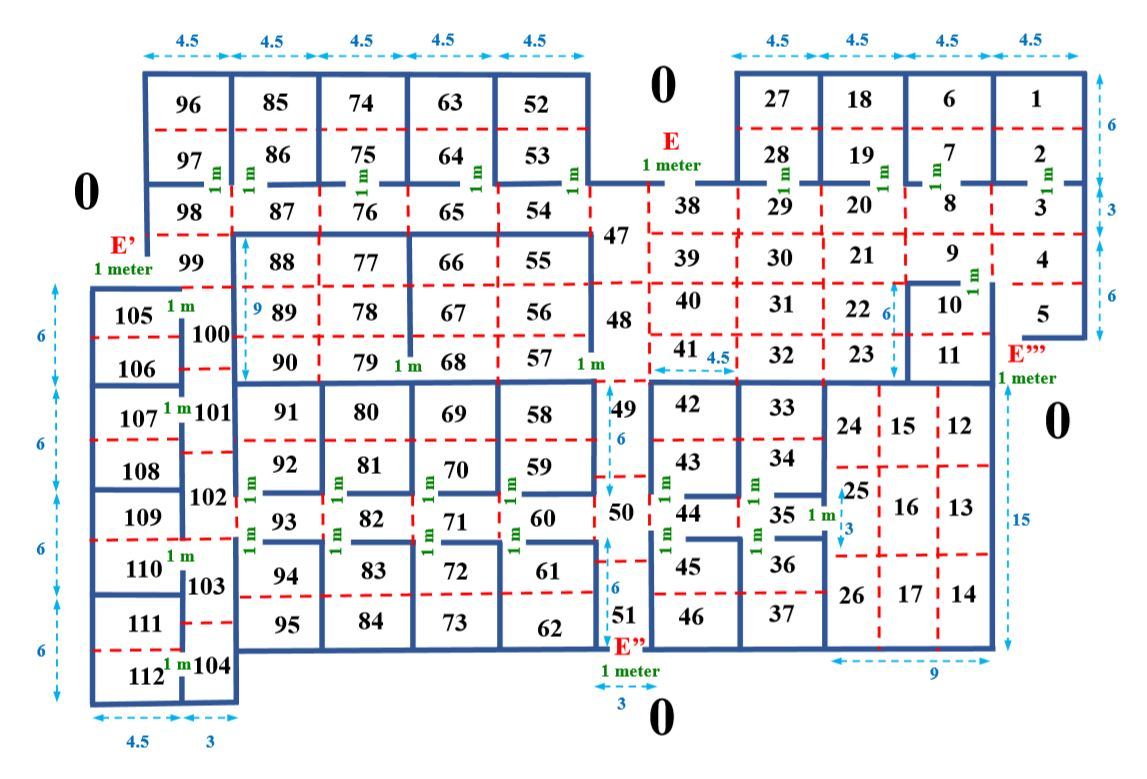
\includegraphics[scale=0.5]{implementation/coppito0.JPG}
	\caption{Coppito 0 Topological Layout}
  \label{Coppito0 layout}
\end{figure}

A detailed description of adaptation of the tool to suit the given scenario is described in the next section.

\section{PedSim Library Modules}
\label{sec: PedSim Library Modules}

The Pedism library allows for the use of pedestrian dynamics into our own software. The libpedsim simulation rendering engine can be extended, modified and modeled to suit specific behavior patterns and scenarios. The above disaster considered is fire and through this thesis, we aim to demonstrate the capabilities of this microscopic simulator, modeling crowds during an emergency evacuation using the above mentioned building topology. 

The implementation of the various scenarios(which will be explained briefly in the following section) using Pedsim is developed on Ubuntu 18.04 using libpedsim version 2.4.2.
The library itself contains many subsections and modules which handle specific tasks such as agent movement, topology description etc. The various modules of the pedsim library is described below.

The libpedsim tool can be broadly classified into 2 sections - the simulation of pedestrians and graphically rendering the simulation process onto a QT based graphical window to depict the flow of agents in real time process.

The following modules are part of rendering output to a graphical window:


\begin{enumerate}
  \item agent.h
  \item agent.cpp
  \item cell.h
  \item cell.cpp
  \item config.h
  \item config.cpp
  \item control.h
  \item control.cpp
  \item control.ui
  \item grid.h
  \item grid.cpp
  \item mainwindow.h
  \item mainwindow.cpp
  \item moc\textunderscore loadscene.cpp
  \item moc\textunderscore control.cpp
  \item moc\textunderscore mainwindow.cpp
  \item moc\textunderscore scene.cpp
  \item moc\textunderscore predefs.cpp
  \item qrc\textunderscore application.cpp
  \item scene.h
  \item scene.cpp
  \item style.h
  \item style.cpp
  \item tree.h
  \item tree.cpp
  \item ui\textunderscore control.h
\end{enumerate}

As the above modules are used to render the algorithm to a graphical output, most of the modules as mentioned above need very little to no modification whatsoever. It is also worth noting that the modules “agent.h” and “agent.cpp” contains the actual definitions for the behavior of pedestrian agents. These behavior functions are implemented by the author of the tool as a generic inter-agent based interaction and is developed keeping in mind to add further and more complex behavioral functionalities. These functions can be extended in the “ped\textunderscore agent.h” and “ped\textunderscore agent.cpp” respectively. 
The following modules below represent the core modules that we extend and modify to suit the scenario at hand:

\begin{enumerate}
  \item coppito.h
  \item coppito.cpp
  \item loadscene.h
  \item loadscene.cpp
  \item ped\textunderscore agent.h
  \item ped\textunderscore agent.cpp
  \item main.cpp
\end{enumerate}

The first two modules - “coppito.h” and “coppito.cpp” is an external module that is incorporated into the source of the libpedsim library for the specific purposes of modeling the building “Coppito 0”, as the name suggests. The detailed description of “coppito.h” and “coppito.cpp” will be listed after the brief description of the other mentioned modules. 

“loadscene” module is used to generate and extract the specific topology of the building. The exact dimensions of the building is stored on an .xml file which is then fed into the loadscene module to incorporate into the library source for graphical representation. This .xml file has specific tags which can be used to not only describe the dimensions of the building but also to specify the number of agents and the path of their trajectory - mentioned as “waypoint” within the .xml file. This information is then retrieved by the loadscene module, extract information from the various mentioned tags, and generating the mentioned number of total agens on the graphical output, adding the constrained waypoints to the agents, and most importantly, to gather the information required to generate a graph that depicts the nature of the building in description.

The “ped\textunderscore agent” module describes the behavior and movement of the agent that is to be rendered to the graphical window. This module consists of behavior functionalities that typically incorporates “social forces”, “obstacle forces”, “look ahead force”, “desired force” and “my force”. The definition of these “forces” (generic navigation constraints and behaviors) are explained below:

\begin{enumerate}
   \item my force:
   \begin{itemize}
     \item myForce() is a method that returns an "empty" force (all components set to 0). This method can be overridden in order to define own forces. This can thus be used to model more complex human navigation/decision making patterns.
   \end{itemize}
   \item lookahead force:
   \begin{itemize}
     \item This calculates the mental layer force of the strategy "look ahead". It is implemented here in the physical layer because of performance reasons.
   \end{itemize}
   \item obstacle force:
   \begin{itemize}
     \item This calculates the force between this agent and the nearest obstacle in this scene.
     \item It iterates over all obstacles.
     \item Hence the complexity of this module is equal to $O(N)$.
   \end{itemize}
   \item social force:
   \begin{itemize}
     \item This module calculates the social force between this agent and all the other agents belonging to the same scene.  It iterates over all agents inside the scene.
     \item Hence it has a complexity of $O(N^2)$.
   \end{itemize}
   \item desired force:
   \begin{itemize}
     \item This module calculates the force between this agent and the next assigned waypoint.  If the waypoint has been reached, the next waypoint in the list will be selected.
     \item At the moment, a visited waypoint is pushed back to the end of the list, which means that the agents will visit all the waypoints over and over again.
   \end{itemize}
\end{enumerate}

The main behavioral functionalities to be incorporated is thus implemented in the ped\textunderscore agent module. The agents are made to move according the complex grid geometry based architecture called \textit{Alan Turing Building Architecture} which is implemented in the “coppito” source module.

As aforementioned, the .xml file contains a generic description of the topology of the building that is to be modeled and used for rendering simulation. The coppito.xml is the file used in our case for the modeling of our present scenario. This information is retrieved by the “loadscene” module to extract the exact graphical plot points to draw the building. 

The following figure \ref{coppito_pedsim} depicts the environment of PedSim and the coppito 0 building that is modeled. 

\begin{figure}[H]
  \centering
  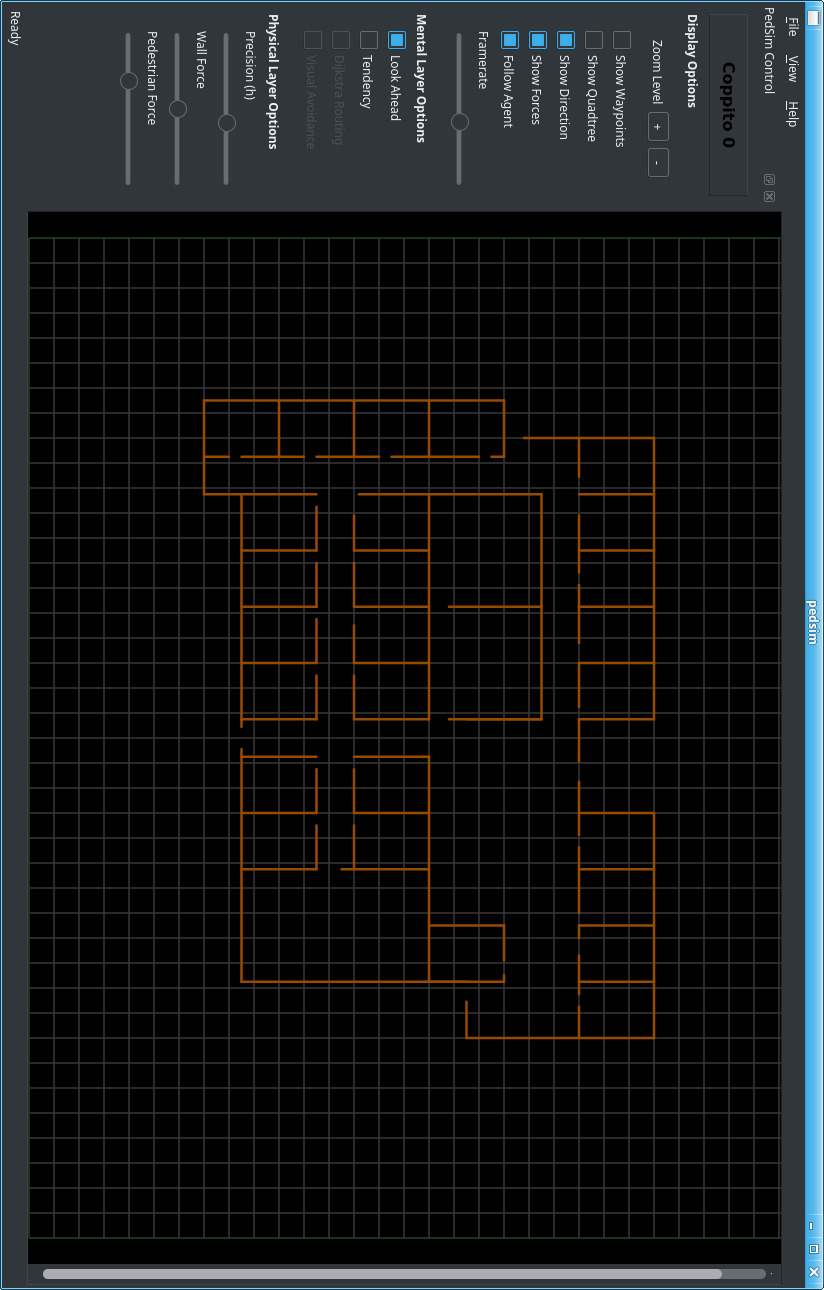
\includegraphics[scale=0.6]{implementation/coppito0building.png}
  \caption{Grid Representation of Coppito 0 within the PedSim Environment}
  \label{coppito_pedsim}
\end{figure}

\begin{figure}[H]
  \centering
  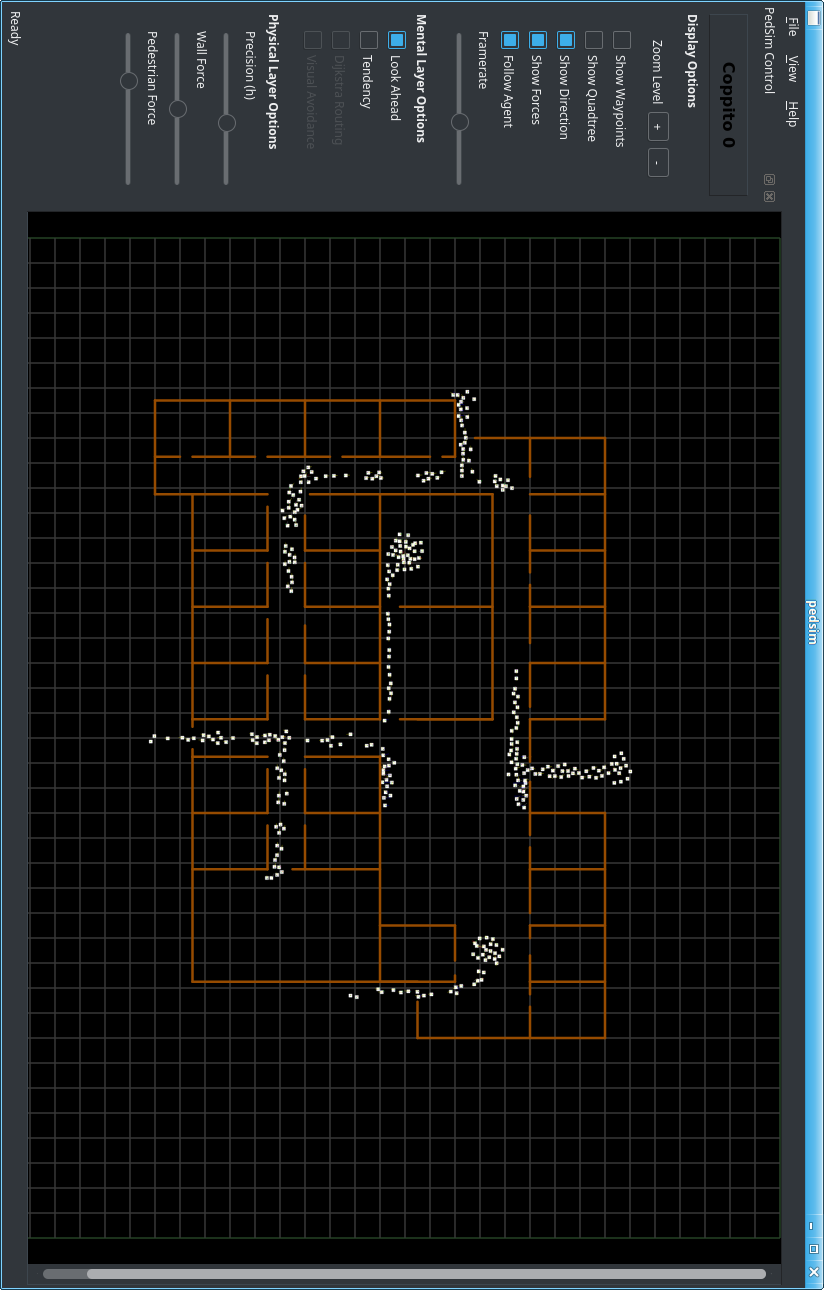
\includegraphics[scale=0.6]{implementation/simulationinaction.png}
  \caption{Microscopic Agent Simulation in PedSim}
  \label{coppito_simulation}
\end{figure}

The above figure \ref{coppito_simulation} represents the microscopic agents being simulated within the PedSim environment, as the agents are subjected to the various constraints and are tasked to evacuate to the safe zone \textbf{"E"}.

PedSim also provides a quick and easy way to change certain key constraints within its front end QT client. The following figure \ref{variableOptions} depicts the variables that can be changed in real time whilst the simulation is being processed.

\begin{figure}[H]
  \centering
  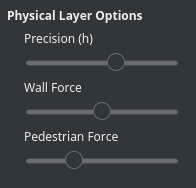
\includegraphics[scale=0.7]{implementation/variableOptions.png}
  \caption{Real Time Variable Constraints in PedSim}
  \label{variableOptions}
\end{figure}

The above figure depicts 3 variable sliders that can be applied to the simulation in real time. The three sliders are explained as follows:

\begin{enumerate}
  \item precision(h) - this represents the time steps $\tau$. These are discretized time steps that are used to calculate the total time taken for the evacuation of the participating agents.
  \item Wall Force - this force determines how close to the obstacles they can tread, this is extremely useful in modelling situations like fire, heat etc., in cases where the walls of the topology should not approached due the nature of the disaster or situation.
  \item Pedastrian Force - This force essentially determines the social forces among the participating agents. The more the pedastrian force the less intermixing happens between the agents. This variable constraint is especially important in modelling cell capacities and in determining flow dynamics. 
\end{enumerate}

The following subsection describes in detail the algorithm that is used in the simulation of the various scenarios. 


\section{Algorithm Description}
\label{sec: Algorithm Description}

All the agents within the PedSim environment are modeled and simulated according to certain realistic constraints. These constraints form the backbone that defines how the agents interact with one another and the environment that surrounds them. To make things simpler, the modeled topology is subdivided into grids. These grids are further divided into atomic square divisions of certain length and breadth. For convenience, we term these square divisions as cells. Constraints such as capacity, flow etc. are imposed on these cells to create a flow dynamic that is closer to the realistic simulation of an emergency evacuation. Within the premise of the running program, these are plot points which are manipulated by the program. 

The “coppito” module pipelines this plot information for further processing. The basic movement of agents are strictly modeled according to the algorithm presented in \cite{ref5}. Various constraints are mentioned in the paper for the anaylsis of a shortest egress path during design time. However these constraints alone are not enough to make the simulations close to be realistic. Once the basic algorithm is explained, further conditions will be introduced and explained. 

In the work by H.Muccini et. al \cite{ref5}, discussion of the linearization of the constraints for effectively reducing the evacuation time of the agents is mentioned. However since its redundant to use linearization within the pedsim framework to simulate for the scenario, we mainly consider only 3 of the below mentioned constraints.

\begin{equation}\label{eq1}
    y^t_j-y^{t-1}_j-\sum_{i:ij\in A}x^{t-1}_{ij}+\sum_{i:ji\in A}x^{t-1}_{ji}=0
\end{equation}

\hspace{100mm} $j\in V,t\in T,t>0$

\begin{equation}\label{eq2}
  0\leq x^t_{ij}+x^t_{ji}\leq c_{ij}
\end{equation}

\hspace{100mm} $t\in T,ij\in A$

\begin{equation}\label{eq3}
  0\leq y^t_i\leq n_i
\end{equation}

\hspace{100mm} $t\in T,i\in V$

Where,

\begin{enumerate}
  \item $T=\{0,1,...,\tau\}$, set of unit of time slots.
  \item $y^t_i$ = state of cell $i\in V$ at time $t\in T$, that is, the number of persons that occupy $i$ at $t$.
  \item $n_i$ = capacity of cell $i$; it measures the maximum nominal amount of people that $i$ can host at any time.
  \item $x^t_{ij}$ = how many persons move from cell $i$ to an adjacent cell $j$ in $(t, t+1]$; this gives the average speed at which the agent flow proceeds from cell $i$ to cell $j$.
  \item $c_{ij}$ = capacity of the passage between cell $i$ and cell $j$; this is the maximum amount of people that, independently on how many persons there are in cell $j$, can traverse the passage in the time unit.
\end{enumerate}

The above conditions are a set of mandatory inclusive pre-requisites required to be included from \textit{An IoT Software Architecture for an Evacuable Building Architecture} by H. Muccini et. al \cite{ref5}, since the experimentation of various scenarios are based on the aforementioned set of equations and conditions. Through this thesis we introduce 4 more constraints to be included along with this base algorithm. The specific nature and details of the additional constraints will be discussed in the next chapter, where the various different experiments and scenarios are carried and are analyzed. It must also be mentioned that in order to be coherent with the mentioned work and also to analyze optimal egress paths the following condition is also considered in addition to the above 3:


\hspace{60mm} max $y^\tau_0$    \hspace{60mm} (3.4)

The above condition is obviously included in order to maximize the number of evacuees during the disaster scenario.


\section{Topology Formulation}
\label{sec: Topology Formulation}


The topology of the building as given in \ref{Coppito0 layout} is modeled according to the \textit{Alan Turing Building Architecture} and as shown in the figure the whole Coppito 0 building is subdivided into cells of equal length and breadth. Each cell also has a cell capacity as defined above and is assumed that inter-connected cells have full passage, if not bound by walls or walls with reduced passage capacity(doors). 

The coppito source module divides the entire topology into such grids that are composed of cells, whose initial plot point is taken from the loadscene module, which in turn takes its information from the coppito.xml file. To translate simple plot points to a complex cell based grid structure, a highly complex user defined data structure was developed to store this information. 

The plot points that are stored into the .xml file is randomly plotted with the exception of the first starting point in order to facilitate a quicker render of the entire building. However for the processing of a cell based structure, this information cannot be random and hence the information is then once again converted to form a structured cell geometry.

Thus a complex user defined data structure is defined to hold all this information in place. For the sake of convenience and optimal storage of data, the coppito 0 building is divided into regions called blocks. Each block contains a set number of cells and naturally have a variable number of cells. The whole topology is divided into 18 blocks and consists in total of 119 cells. Each cell is also of a specific dimension and has a certain cell length and a cell width. To understand what a block is, it can be easily explained diagrammatically as follows:

\begin{figure}[H]
  \centering
  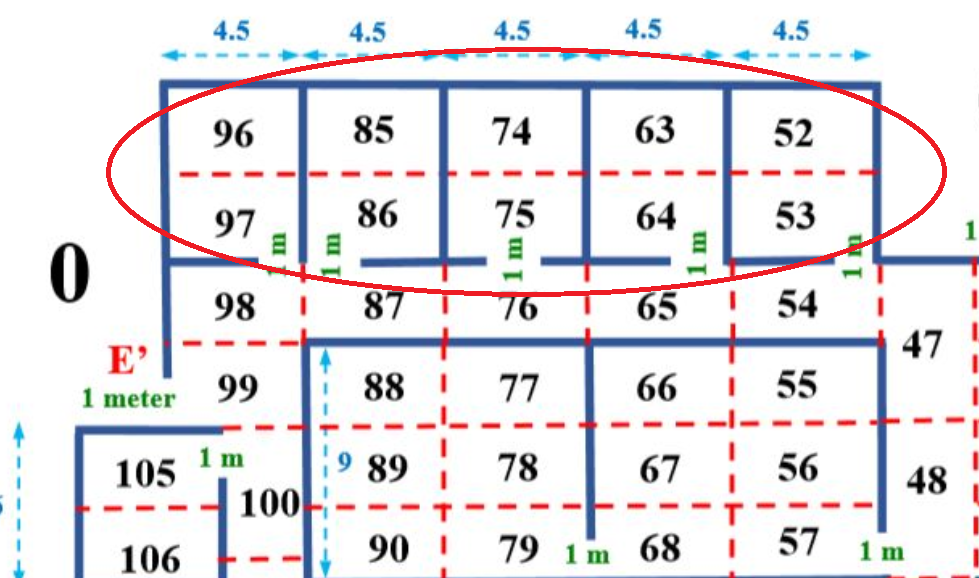
\includegraphics[scale=0.5]{implementation/block.png}
  \caption{Groups of Cells Making a Block Structure}
  \label{block}
\end{figure}

From the above figure \ref{block}, the red encircled circled area which includes the cells numbered 96, 85, 74, 63, 52, 97, 86, 75, 64, 53 form a block. Although a certain number of cells make up a block, the number of cells that make a block is often variable. Essentially one section of the topology is considered a block. This helps segregate different areas of the premises and identify them easily.

Further decomposing the cell, subdivides it into 4 edge lines, each edge line further decomposes into 4 vertices, an end to end $x$ and $y$ plot points. Along with these information are stored if the edge lines are walls and if they incorporate doors. This is highly useful for creating a tree structure pattern for path finding, used by agents during evacuation simulation. The final complex structure that is defined to hold this cell structure is explained in detail in the Appendix section. In order to dynamically store the data of the cell information, the data structure used in place is a custom user defined 7 layered structure. 

There are several sub-modules implemented in this custom made source file. The following are the following methods that are implemented as part of the module:

\begin{enumerate}
  \item divide\textunderscore cells
  \item cell\textunderscore structure\textunderscore allocation
  \item vertical\textunderscore cell\textunderscore allocation
  \item non\textunderscore standard\textunderscore vertical\textunderscore allocation
  \item wall\textunderscore allocation
  \item wall\textunderscore division\textunderscore horizontal
  \item wall\textunderscore division\textunderscore vertical
  \item door\textunderscore allocation
  \item graph\textunderscore tree\textunderscore structuring
  \item print\textunderscore block
  \item print\textunderscore walls
  \item print\textunderscore door
  \item print\textunderscore graph
\end{enumerate}

Further details regarding the technical and programmatic implementation of these modules are provided in the Appendix section of the thesis. The following section discusses the modification to the existing unoptimized algorithm from \cite{ref5}. The different simulation results comparing macro and micro agent simulations are presented and analyzed. The resulting the implications of these observations are discussed. 
 


 \chapter{Experimentation and Analysis\label{ch:Experimentation and Analysis}}

This chapter is intended to provide the experimental proof of the proposed extension of the previously formulated algorithm from \cite{ref5}. Through this chapter, the detailed explanation of the additional constraints that are added to the unoptimized simulation from the previous chapter is provided. Next micro and macro agent simulations are presented pertaining to certain cases and scenarios to compare between the unoptimized and the optimized simulations. The resulting observations and statistics are then presented for further analysis and the implications are then discussed.

\section{Optimization through Constraints}
\label{sec: Optimization through Constraints}

From the equations \ref{eq1}, \ref{eq2} and \ref{eq3}, the basic conditions for agent occupancy, flow control and cell capacity is discussed. However these conditions are hardly realistic when compared to modelling a real crowd of agents. In realistic scenarios, groups of people have altered behavior, confusion panic etc. There will be different forms of social constraints, varying movement speeds, and due to the impaired cognition, perceptions can change leading to different decisions that are made during a catastrophe. To model some of these realistic scenarios, it became evident that the inclusion of certain more properties to the scenario was mandatory. The following conditions as mentioned in section \ref{sec:intro:Objectives and Approach} is analyzed here:

\begin{enumerate}
  \item Cell capacity specification by defining social distances
  \begin{itemize}
  	\item Although PedSim comes by default with a cell class, it does not go coherently with the topology, as cell divisions are highly subjective and can change their length and breadth according to the defined scenario. To cater for this, manipulation of the social forces constraint causes agents to maintain a certain "social distance" from each other. This can be used to our advantage to simulate cell capacities based on these social distances.
  \end{itemize}
  \item Definition of total area capacity and doors flow capacity constraints -congestion control
  \begin{itemize}
  	\item The simulation present \cite{ref5}, unfortunately does not present the congestion scenario as well due to the simplistic constraints present. Providing additional constraint for area capacity, door flow capacity and passageway capacity can help reduce congestion and enable the re-routing of agents to alternate exits or routes in real time.
  \end{itemize}
  \item Simulating social attachment among some agents
  \begin{itemize}
  	\item With the introduction of the group constraint, social attachments can be modeled for a more realistic approach. For instance friends move together, a mother will most likely not be separable from her child etc. These groups can be defined during the simulation and then observed for the various real time decisions that these groups of agents make.
  \end{itemize}
  \item Setting the speed accordingly for various groups
  \begin{itemize}
  	\item By default PedSim models for microscopic agents and hence the entirety of the agents are considered as a single group. The movement speed for these agents are varied across a distribution and the average speed set for the microscopic group of agents. By setting a variable speed constraint and with the introduction of groups, we model PedSim to cater for macro and micro agent simulation and thus support varying speeds according to the different group formations that can be defined during the simulation. In other words $v_{max}$ is not fixed across all agents.
  \end{itemize}
\end{enumerate}

The PedSim library is extended to be inclusive of the algorithm from the section \ref{sec: Algorithm Description} and the aforementioned constraints in order to simulate the various scenarios for micro and macro agents. The following section provides a detailed analysis of the various scenarios that are simulated within the PedSim environment.  

\section{Simulation and Scenario Analysis}
\label{sec: Simulation and Scenario Analysis}

This section contains the experimental analysis based on the scenarios that are presented in the forthcoming subsections. It must be noted that the following simulations are run on a PC with the following specifications - Ubuntu 18.04, 8 GB ram, and an i5 processor with 2.5 ghz clock speed. A series of sub-sections are present in this section - each representing a particular scenario for simulation. The scenario will be described and the corresponding tabular observations and graph is then presented. 

There are some properties that are common to scenarios. We follow similar topological constraints as given in \cite{ref5}. For instance, in the previous work presented, the cells are assumed to be isometric, i.e. the cells are bi-directional and can be crossed from any direction with the same amount of time. In the scenarios presented, the cells are assumed to be isometric as well.

According to the work by Daamen et al. \cite{ref23}, door capacities are presented, where they are based on varying stress and composition levels of agents and he subesquently proposes an average of 2.8 persons per second for a 1 meter wide door $(p/m/s)$. In order to perform a statistical analysis and to remain coherent with the results with from \cite{ref5}, the door capacities and cell capacities are modeled after the presented stats in the aforementioned work. In \cite{ref5} the pessimistic and optimistic values considered are 1.03 $p/m/s$ and 3.23 $p/m/s$ respectively. This translates to a maximum of 5 people in pessimistic and a maximum of 16 people in optimistic situation can pass through a 1 meter wide door per slot time (5 seconds). Hence the same values will be considered here as well. There are also a certain terms that are used in this section, namely, optimistic and pessimistic. Optimistic scenario assumes that no passageways and exits are blocked. Whereas pessimistic scenario assumes that 50\% of the emergency exits are blocked and passageways can accommodate only 5 people at a time. 

The maximum number of people considered is 1008, as mentioned in \cite{ref5}. All the above conditions are compliant with the mentioned paper.

\subsection{Case 1: Macro Agent Simulation Comparing Optimized and Un-Optimized Simulations}
\label{sec: Case 1: Macro Agent Simulation Comparing Optimized and Un-Optimized Simulations}

The first case is depicts the CPU run time comparison between macro agents(single or no group concept is present here) that follow the optimized algorithm from \cite{ref5} against the proposed extension of the simulation by additional constraints. For the current scenario, pessimistic path scenario is incorporated in order to keep the coherency of results and perform the necessary comparisons with the aforementioned paper.

A total of 1008 people are taken for the purposes of this simulation. Various walking speed scenarios among acquintances and friendly dyads are presented in the work by Wagnild et al. \cite{ref24}, however since there are no complex group formations that are currently part of the simulation, the speed of 1.2 $m/s$ estimated in J. Ye's average \textit{free flowing walking velocity} \cite{ref25} is used here.

The original code for simulation was written on OPL language and solved on CPLEX version 12.8.0 \cite{ref5}. However codebase for the modified algorithm has since been translated to the PedSim environment. The following table \ref{Macro Agent Simulation - Optimized vs UnOptimized Simulation} represents the simulation times between the optimized and the un-optimized modeling scenarios.
 

\begin{table}[H]
\centering
\begin{adjustbox}{angle=270}
\scalebox{0.7}{
\begin{tabular}{|l|l|l|l|l|l|l|l|} 
\hline
\textcolor[rgb]{0.133,0.133,0.133}{τ} & Evacuees & CPU Time (sec) - Optimized & CPU Time (sec) - Un-Optimized & \textcolor[rgb]{0.133,0.133,0.133}{τ} & Evacuees & CPU Time (sec) - Optimized & CPU Time (sec) - Un-Optimized  \\ 
\hline
1                                     & 20       & 0.25                       & 0.28                         & 27                                    & 540      & 4.9                        & 2.61                          \\
2                                     & 40       & 0.28                       & 0.31                         & 28                                    & 560      & 5.1                        & 2.77                          \\
3                                     & 60       & 0.47                       & 0.44                         & 29                                    & 580      & 5.7                        & 2.84                          \\
4                                     & 80       & 0.61                       & 0.53                         & 30                                    & 600      & 6                          & 2.96                          \\
5                                     & 100      & 0.63                       & 0.47                         & 31                                    & 620      & 6.5                        & 3.1                           \\
6                                     & 120      & 0.69                       & 0.58                         & 32                                    & 640      & 6.94                       & 3.53                          \\
7                                     & 140      & 0.72                       & 0.6                          & 33                                    & 660      & 7.2                        & 3.32                          \\
8                                     & 160      & 0.75                       & 0.61                         & 34                                    & 680      & 7.76                       & 3.54                          \\
9                                     & 180      & 0.82                       & 0.71                         & 35                                    & 700      & 7.96                       & 3.91                          \\
10                                    & 200      & 0.88                       & 0.76                         & 36                                    & 720      & 8.4                        & 3.42                          \\
11                                    & 220      & 1.1                        & 0.83                         & 37                                    & 740      & 8.7                        & 4.14                          \\
12                                    & 240      & 1.22                       & 0.88                         & 38                                    & 760      & 9.3                        & 4.16                          \\
13                                    & 260      & 1.27                       & 1.01                         & 39                                    & 780      & 9.88                       & 4.17                          \\
14                                    & 280      & 1.33                       & 1.09                         & 40                                    & 800      & 10.4                       & 4.19                          \\
15                                    & 300      & 1.4                        & 1.12                         & 41                                    & 820      & 10.79                      & 4.3                           \\
16                                    & 320      & 1.6                        & 1.44                         & 42                                    & 840      & 11.5                       & 5.13                          \\
17                                    & 340      & 1.82                       & 1.28                         & 43                                    & 860      & 12.37                      & 5.07                          \\
18                                    & 360      & 1.99                       & 1.33                         & 44                                    & 880      & 13.01                      & 5.12                          \\
19                                    & 380      & 2.1                        & 1.57                         & 45                                    & 900      & 13.68                      & 5.27                          \\
20                                    & 400      & 2.3                        & 1.61                         & 46                                    & 920      & 14.5                       & 5.36                          \\
21                                    & 420      & 2.44                       & 1.73                         & 47                                    & 940      & 15.4                       & 5.49                          \\
22                                    & 440      & 2.6                        & 1.88                         & 48                                    & 960      & 16.04                      & 6.01                          \\
23                                    & 460      & 2.9                        & 2.02                         & 49                                    & 980      & 17.07                      & 6.35                          \\
24                                    & 480      & 3.3                        & 2.08                         & 50                                    & 1000     & 18.2                       & 6.25                          \\
25                                    & 500      & 3.8                        & 2.19                         & 51                                    & 1008     & 19.4                       & 6.47                          \\
26                                    & 520      & 4.4                        & 2.35                         &                                       &          &                            &                               \\
\hline
\end{tabular}}
\end{adjustbox}
\caption{Macro Agent Simulation - Optimized vs UnOptimized Simulation}
\label{Macro Agent Simulation - Optimized vs UnOptimized Simulation}
\end{table}

It is evident from the above figure that the optimized algorithm takes an exponential time to compute the simulation times for the macro agents at the given number of time steps. Below is a graphical description of the observed statistical values from the table \ref{Macro Agent Simulation - Optimized vs UnOptimized Simulation}.

\begin{figure}[H]
  \centering
  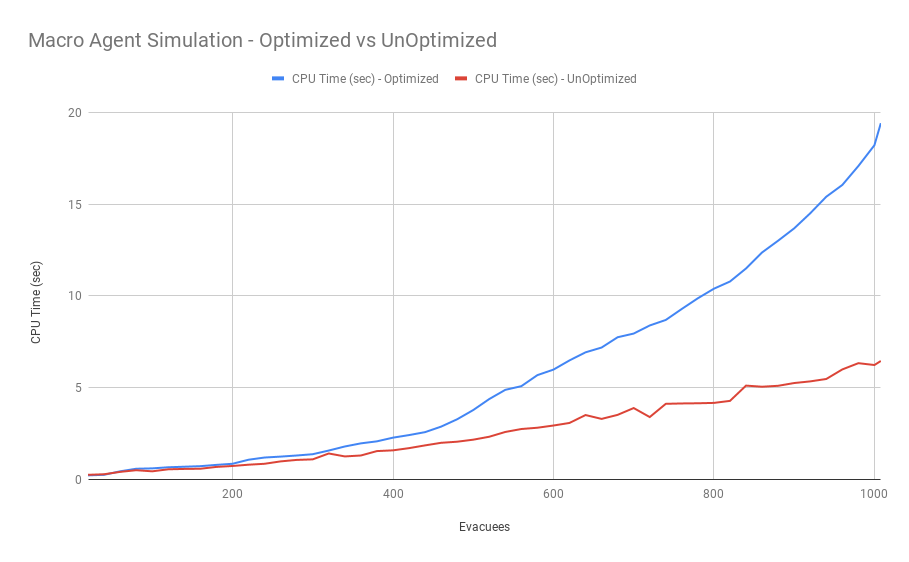
\includegraphics[scale=0.5]{simulation/Macro_Agent_Simulation.png}
  \caption{Macro Agent Simulation - Optimized vs UnOptimized Simulation}
  \label{Macro Agent Simulation}
\end{figure}

The above figure \ref{Macro Agent Simulation} depicts the difference in the performance experienced as the constraints placed are higher in count and complexity. In the present scenario, not all the constraints are incorporated however. In macro agent simulation, no grouping is employed, hence there is no grouping constraint. This in turn also affects the varying speed constraint as groups of agents are not involved. It is also noteworthy mentioning that single agents can be considered as individual groups as well. Since there is no such constraint, the average of 1.2 $m/s$ velocity for all agents is applied and the simulation of the agents are then performed.


\subsection{Case 2: Run Time Comparison between Micro and Macro Agent Simulation}
\label{sec: Case 2: Run Time Comparison between Micro and Macro Agent Simulation}

This case is similar in terms of objective to the previous case \ref{sec: Case 1: Macro Agent Simulation Comparing Optimized and Un-Optimized Simulations}. However the key difference lies in what is compared in this particular scenario. Micro and macro agent simulation scenarios are compared in this case. Since there is micro agents that are also included, grouping constraints are included and subsequently varying velocities based on grouping and affiliation.

\subsubsection{Statistical Purview of Gait Speeds Among People}
\label{sec: Statistical Purview of Gait Speeds Among People}
To understand the how human walking speed impacts the simulation performance and the overall evacuation time, the work presented by Simonsick et al. \cite{ref29} is used as a baseline agent walking speed reference. The work presents an extensive statistical review on the walking speeds of people across all ages and sex. The walking speeds of people, according to Simonsick et al., is based on a variety of factors. These factors include not only a generic health purview and disabilities, but other social and psychological factors such as education and lifestyle. The factors that are taken into account are age, sex, education, marital status, smoker/non-smoking lifestyle, comorbidity, subjective health, waist circumference, height, neuroticism, extraversion openness, agreeableness, conscientiousness, systolic and diastolic BP, cholesterol levels, triglyceride levels, handgrip strength, averge walking activity per week etc. 

The following statistical graphs were obtained based on their analysis and observations as given in \cite{ref29}:

\begin{figure}[H]
\subfloat[fig a]{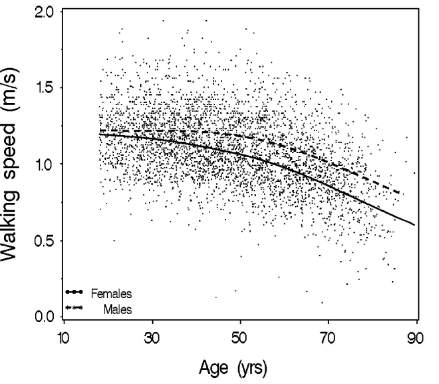
\includegraphics[width = 3in]{simulation/1.png}} 
\subfloat[fig b]{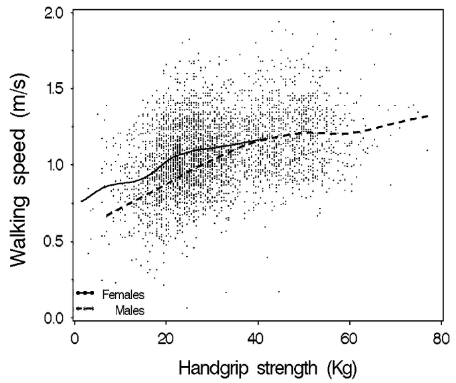
\includegraphics[width = 3in]{simulation/2.png}}\\
\subfloat[fig c]{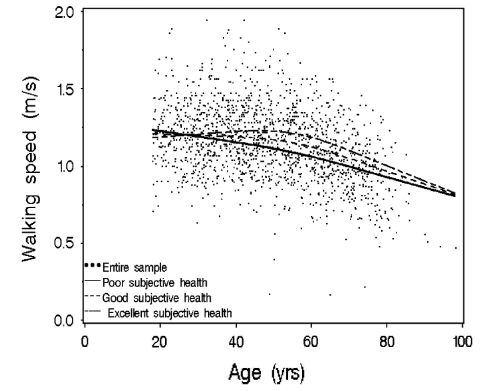
\includegraphics[width = 3in]{simulation/3.png}}
\subfloat[fig d]{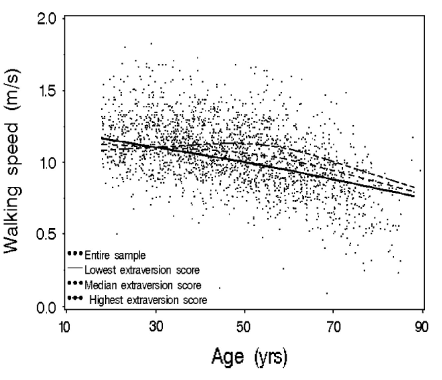
\includegraphics[width = 3in]{simulation/4.png}} 
\caption{Walking Speed Statistics}
\label{Walking Speed Statistics}
\end{figure}

The above figure presents the walking speeds of people based on a few of the aforementioned factors. According to the study, the age of 55 was considered as the inflection point for walking speed sensitivity. All the statistical models hence were modeled considering 55 as the age of inflection. Generally the study found out that women walked slower than men at all ages, with more pronounced variations after the age of 55. Younger women walked faster than the older women. According to the study, the walking speed varied from 0.7 to 1.2 $m/s$.

Another study was performed by Wagnild et al. \cite{ref24}, and he determined that walking speeds are highly depend on the company and the lowest speed of the person present in the group. This scenario is inclusive of group constraints. However this scenario is also only to compare the actual running times of the simulated output. Complexities regarding group dynamics are not compared here. To keep the results coherent, the macro agents are considered with the uniform speed as mentioned in the previous section. The micro agents consists of mixed groups and individuals. 

To present the impact of walking speeds in an evacuation scenario, the following graph depicts the evacuation time required in the case of variation of walking speeds of people who move slower than the average speed during an evacuation. In this scenario however, macra agent model is considered. The simulation trial is run with the same optimized algorithm from \cite{ref5}. The total number of agents considered in the following scenario is $N = 1008$.

\begin{figure}[H]
  \centering
  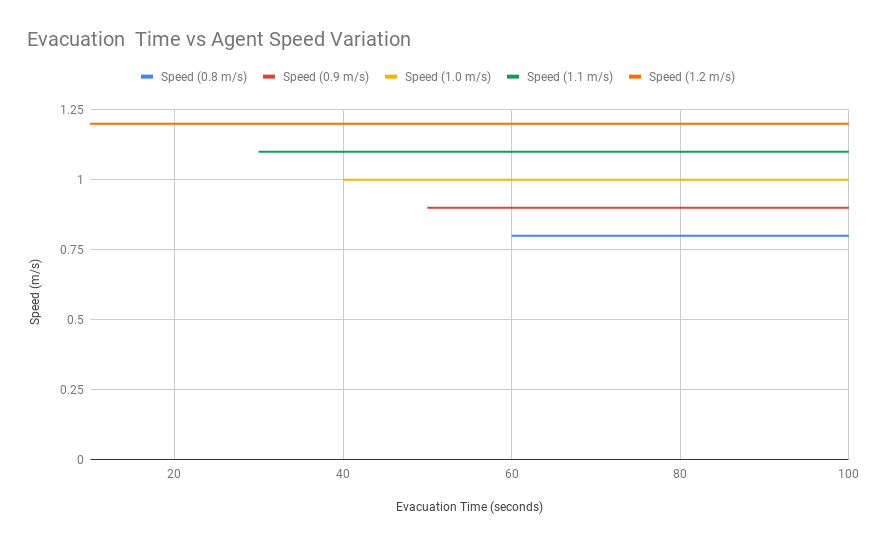
\includegraphics[scale=0.5]{simulation/EvacuationTimevsAgentSpeedVariation.png}
  \caption{Evacuation Time vs Agent Speed Variation}
  \label{Evacuation Time vs Agent Speed Variation}
\end{figure}

In the given figure \ref{Evacuation Time vs Agent Speed Variation}, it is explicitly shown how walking speeds directly affect the total evacuation time of the agents during a disaster event.

\subsubsection{Computation Time - Micro vs Macro Agent Simulation}
\label{sec: Computation Time - Micro vs Macro Agent Simulation}

The comparison values are based off on the pessimistic path scenario as presented in \cite{ref5}. A cross way comparison between macro agents with un-optimized simulation constraints, macro agents simulated with optimized constraints and micro agent with constraints is tabulated in the table below. The CPU run time values for the microscopic agents that are simulated using the un-optimzed are obtained from the charted values from table 2.0 from the aforementioned paper, based on which the other two comparisons can be made and analyzed. To keep group velocity diversity among the micro agents, 20\% of the total number of micro agents are randomly distributed with varying speeds between the range of 0.7 $m/s$ and 1.2 $m/s$.

A total number of evacuees upto 1008 are considered for the comparisons, similar to the previous section \ref{sec: Case 1: Macro Agent Simulation Comparing Optimized and Un-Optimized Simulations}. 

\begin{table}
\centering
\begin{adjustbox}{angle=270}
\scalebox{0.7}{
\begin{tabular}{|l|l|l|l|} 
\hline
Evacuees & CPU Time (sec) - Macro Agent Sim:Optimized with Constraints & Evacuees & CPU Time (sec) - Micro Agent Sim:Optimized with Constraints  \\ 
\hline
20       & 0.4                                                         & 540      & 10.8                                                         \\
40       & 0.46                                                        & 560      & 11.5                                                         \\
60       & 0.6                                                         & 580      & 12.3                                                         \\
80       & 0.8                                                         & 600      & 13.8                                                         \\
100      & 0.9                                                         & 620      & 14.97                                                        \\
120      & 1.01                                                        & 640      & 15.92                                                        \\
140      & 1.11                                                        & 660      & 17.3                                                         \\
160      & 1.4                                                         & 680      & 19.2                                                         \\
180      & 1.7                                                         & 700      & 21.84                                                        \\
200      & 2                                                           & 720      & 23.7                                                         \\
220      & 2.3                                                         & 740      & 25.9                                                         \\
240      & 2.4                                                         & 760      & 27.9                                                         \\
260      & 2.7                                                         & 780      & 30.2                                                         \\
280      & 3.2                                                         & 800      & 33.5                                                         \\
300      & 3.5                                                         & 820      & 36.7                                                         \\
320      & 3.9                                                         & 840      & 39                                                           \\
340      & 4.3                                                         & 860      & 43.3                                                         \\
360      & 4.8                                                         & 880      & 47.2                                                         \\
380      & 5.4                                                         & 900      & 50.34                                                        \\
400      & 5.9                                                         & 920      & 54.2                                                         \\
420      & 6.5                                                         & 940      & 58.99                                                        \\
440      & 6.97                                                        & 960      & 64.2                                                         \\
460      & 7.6                                                         & 980      & 68.2                                                         \\
480      & 8.1                                                         & 1000     & 74.78                                                        \\
500      & 8.7                                                         & 1008     & 76.34                                                        \\
520      & 9.7                                                         &          &                                                              \\
\hline
\end{tabular}}
\end{adjustbox}
\caption{CPU Time Comparison between Micro and Macro Agent Simulation}
\label{CPU Time Comparison between Micro and Macro Agent Simulation}
\end{table}  

As it can be noted from the above table \ref{CPU Time Comparison between Micro and Macro Agent Simulation}, the time taken for the micro agent simulation far exceeds the time taken by both the previous simulations - for macro agent model in both optimized and un-optimized simulations. However, it should be noted that the micro agent simulation has 20\% of the entire participants at a reduced movement speed, during each simulation run. Since the number of reduced movement speed agents increase exponentially for each trial run, so does the computation time. These agents who have reduced speeds are also randomized to form certain affliate bonds and groups. 

More discussion on the nature of such groups and their implications are discussed in the next sub-section where the evacuation time is discussed in detail and simulations are run in order to observe the actual time taken due to the additional constraints.

The below figure \ref{Micro vs Macro Agent Simulation} represents the comparison between the 3 major simulation models and their exceedingly apparent ranges of computation times. 

\begin{figure}[H]
  \centering
  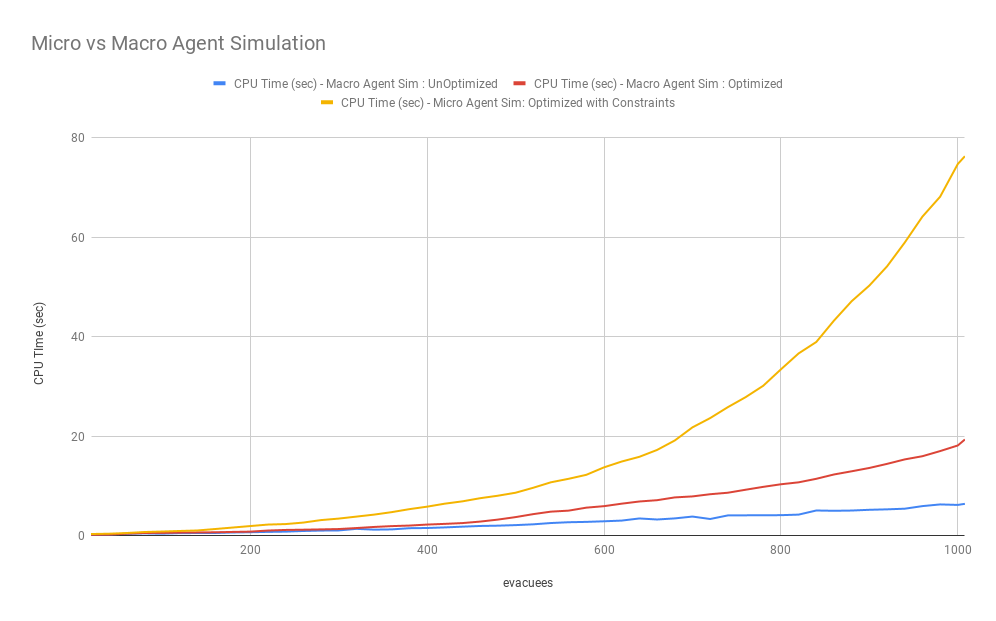
\includegraphics[scale=0.47]{simulation/Micro_vs_Macro_Agent_Simulation.png}
  \caption{Micro vs Macro Agent Simulation}
  \label{Micro vs Macro Agent Simulation}
\end{figure}

From the figure, the following inferences can be made:

\begin{enumerate}
  \item The macro agent simulation with no constraints and simulated according to the base algorithm and a constant $v_{max}$ movement velocity has a time complexity of $O(N)$.
  \item The macro agent simulation subjected to constraints such as social force definition, area capacity and flow capacity, exhibit a time complexity of $O(N^2)$.
  \item Micro agent simulation subjected to varying speeds and grouping in addition to social forces and flow capacity definition for congestion control, exhibit a time complexity of $O(N^3)$.
\end{enumerate}

The implications for these inferences will be discussed in section 4.3.


\subsection{Case 3: Congestion Dynamics and Flow Control}
\label{sec: Case 3: Congestion Dynamics and Flow Control}

This section presents a detailed case on the effect of the width of emergency exits on the evacuation time. The work by H. Muccini et al. \cite{ref5} focuses on an ideal and optimal path without accounting for more advanced constraints. One of the most important effects of a disaster on human agents is the element of chaos and panic. This causes most agents to panic and make rash decisions, all clustering towards an exit point. This causes massive congestions and jams which ultimately leads to stampedes and also the failure for the agents to evacuate to an exist point in the shortest time frame possible. To analyze an optimal egress path however, we do not simulate congestion itself as such, rather we aim for congestion avoidance. To avoid congestion, the routes for various people need to be calculated in real time in order to re-route in the case of an impending congestion scenario.

In order to analyze the congestion, we must first answer the question, what leads to congestion? The answer is two fold as follows:
\begin{itemize}
  \item The obvious answer is - too little space and too many people to fill that space. The forthcoming tables and graphs are to experiment the effect of exit width on congestion.
  \item The second answer is more complex, dealing with walking speeds, social forces and group decisions. 
\end{itemize}

In section \ref{sec: Case 4: Shortest Path vs Ideal Path}, detailed case study on walking speeds and decision making is presented. Although the same group dynamics applies to this case too, the focus is on exit width. The forthcoming tables and graph depict the various scenarios that are simulated for both macro and micro agents using the un-optimized and optimized algorithms respectively.

The following table \ref{Emergency Exits Width vs Evacuation Time : Optimistic Values for Macro Agent Model} depicts optimistic values for macro agents whilst varying exit capacities and thus in turn affecting flow dynamics.

\begin{table}[H]
\centering
\scalebox{0.7}{
\begin{tabular}{|l|l|l|} 
\hline
Emergency Exit Width (m) & \begin{tabular}[c]{@{}l@{}}Evacuation Time Horizon $(\tau)$ - \\Optimistic values for \\Unoptimized Simulation\end{tabular} & \begin{tabular}[c]{@{}l@{}}Evacuation Time Horizon $(\tau)$ - \\Optimistic Values for \\Optimized Simulation\end{tabular}  \\ 
\hline
0.4                      & 45                                                                                                                  & 83                                                                                                                 \\
0.5                      & 43                                                                                                                  & 79                                                                                                                 \\
0.6                      & 37                                                                                                                  & 76                                                                                                                 \\
0.7                      & 33                                                                                                                  & 73                                                                                                                 \\
0.8                      & 28                                                                                                                  & 70                                                                                                                 \\
0.9                      & 25                                                                                                                  & 68                                                                                                                 \\
1.0                      & 22                                                                                                                  & 62                                                                                                                 \\
1.1                      & 20                                                                                                                  & 58                                                                                                                 \\
1.2                      & 16                                                                                                                  & 53                                                                                                                 \\
1.3                      & 12                                                                                                                  & 48                                                                                                                 \\
1.4                      & 11                                                                                                                  & 45                                                                                                                 \\
1.5                      & 10                                                                                                                  & 40                                                                                                                 \\
1.6                      & 9                                                                                                                   & 37                                                                                                                 \\
1.7                      & 9                                                                                                                   & 32                                                                                                                 \\
1.8                      & 8                                                                                                                   & 29                                                                                                                 \\
1.9                      & 7                                                                                                                   & 25                                                                                                                 \\
2.0                      & 6                                                                                                                   & 20                                                                                                                 \\
2.1                      & 5                                                                                                                   & 18                                                                                                                 \\
2.2                      & 5                                                                                                                   & 15                                                                                                                 \\
2.3                      & 5                                                                                                                   & 12                                                                                                                 \\
2.4                      & 4                                                                                                                   & 8                                                                                                                  \\
2.5                      & 3                                                                                                                   & 6                                                                                                                  \\
2.6                      & 3                                                                                                                   & 5                                                                                                                  \\
2.7                      & 3                                                                                                                   & 3                                                                                                                  \\
2.8                      & 2                                                                                                                   & 2                                                                                                                  \\
2.9                      & 2                                                                                                                   & 2                                                                                                                  \\
3.0                      & 1                                                                                                                   & 1                                                                                                                  \\
\hline
\end{tabular}}
\caption{Emergency Exits Width vs Evacuation Time : Optimistic Values for Macro Agent Model}
\label{Emergency Exits Width vs Evacuation Time : Optimistic Values for Macro Agent Model}
\end{table}

Comparison between the pessimistic cases of optimized and the un-optimized cases are presented for macro agent model below in table \ref{Emergency Exits Width vs Evacuation Time : Pessimistic values for Macro Agent Simulation}:


\begin{table}[H]
\centering
\scalebox{0.7}{
\begin{tabular}{|l|l|l|} 
\hline
    Emergency Exit Width (m) & \begin{tabular}[c]{@{}l@{}}Evacuation Time Horizon $(\tau)$ -\\Pessimistic Values for \\UnOptimized Simulation\end{tabular} & \begin{tabular}[c]{@{}l@{}}Evacuation Time Horizon $(\tau)$ -\\Pessimistic Values for \\Optimized Simulation\end{tabular}  \\ 
\hline
0.4                      & 120                                                                                                                 & 205                                                                                                                \\
0.5                      & 105                                                                                                                 & 192                                                                                                                \\
0.6                      & 94                                                                                                                  & 181                                                                                                                \\
0.7                      & 86                                                                                                                  & 173                                                                                                                \\
0.8                      & 76                                                                                                                  & 163                                                                                                                \\
0.9                      & 68                                                                                                                  & 155                                                                                                                \\
1.0                      & 62                                                                                                                  & 140                                                                                                                \\
1.1                      & 56                                                                                                                  & 127                                                                                                                \\
1.2                      & 53                                                                                                                  & 111                                                                                                                \\
1.3                      & 48                                                                                                                  & 101                                                                                                                \\
1.4                      & 45                                                                                                                  & 93                                                                                                                 \\
1.5                      & 42                                                                                                                  & 80                                                                                                                 \\
1.6                      & 37                                                                                                                  & 72                                                                                                                 \\
1.7                      & 33                                                                                                                  & 65                                                                                                                 \\
1.8                      & 29                                                                                                                  & 52                                                                                                                 \\
1.9                      & 25                                                                                                                  & 47                                                                                                                 \\
2.0                      & 20                                                                                                                  & 30                                                                                                                 \\
2.1                      & 18                                                                                                                  & 19                                                                                                                 \\
2.2                      & 15                                                                                                                  & 17                                                                                                                 \\
2.3                      & 12                                                                                                                  & 14                                                                                                                 \\
2.4                      & 8                                                                                                                   & 11                                                                                                                 \\
2.5                      & 6                                                                                                                   & 8                                                                                                                  \\
2.6                      & 5                                                                                                                   & 6                                                                                                                  \\
2.7                      & 3                                                                                                                   & 5                                                                                                                  \\
2.8                      & 2                                                                                                                   & 3                                                                                                                  \\
2.9                      & 2                                                                                                                   & 2                                                                                                                  \\
3.0                      & 1                                                                                                                   & 1                                                                                                                  \\
\hline
\end{tabular}}
\caption{Emergency Exits Width vs Evacuation Time : Pessimistic values for Macro Agent Simulation}
\label{Emergency Exits Width vs Evacuation Time : Pessimistic values for Macro Agent Simulation}
\end{table}

To run a simulation for the case of micro model agents, certain characteristics were given to 20\% of the total number of agents in each case. The characteristics include variable speeds(random speed between 0. 7 $m/s$ and 1.4 $m/s$), and the other constraints of area capacity and the variable exit door capacity as follows:


\begin{table}[H]
\centering
\scalebox{0.7}{
\begin{tabular}{|l|l|l|} 
\hline
Emergency Exit Width (m) & \begin{tabular}[c]{@{}l@{}}Evacuation Time Horizon $(\tau)$ - \\Optimistic Values for \\Micro Agent Simulation\end{tabular} & \begin{tabular}[c]{@{}l@{}}Evacuation Time Horizon $(\tau)$ - \\Pessimistic Values for \\Micro Agent Simulation\end{tabular}  \\ 
\hline
0.4                      & 246                                                                                                                  & 415                                                                                                                    \\
0.5                      & 223                                                                                                                  & 370                                                                                                                    \\
0.6                      & 202                                                                                                                  & 340                                                                                                                    \\
0.7                      & 192                                                                                                                  & 306                                                                                                                    \\
0.8                      & 184                                                                                                                  & 292                                                                                                                    \\
0.9                      & 178                                                                                                                  & 270                                                                                                                    \\
1.0                      & 155                                                                                                                  & 240                                                                                                                    \\
1.1                      & 140                                                                                                                  & 212                                                                                                                    \\
1.2                      & 129                                                                                                                  & 193                                                                                                                    \\
1.3                      & 111                                                                                                                  & 163                                                                                                                    \\
1.4                      & 101                                                                                                                  & 140                                                                                                                    \\
1.5                      & 85                                                                                                                   & 124                                                                                                                    \\
1.6                      & 74                                                                                                                   & 112                                                                                                                    \\
1.7                      & 65                                                                                                                   & 99                                                                                                                     \\
1.8                      & 51                                                                                                                   & 83                                                                                                                     \\
1.9                      & 48                                                                                                                   & 60                                                                                                                     \\
2.0                      & 31                                                                                                                   & 47                                                                                                                     \\
2.1                      & 19                                                                                                                   & 33                                                                                                                     \\
2.2                      & 16                                                                                                                   & 28                                                                                                                     \\
2.3                      & 13                                                                                                                   & 20                                                                                                                     \\
2.4                      & 10                                                                                                                   & 16                                                                                                                     \\
2.5                      & 8                                                                                                                    & 9                                                                                                                      \\
2.6                      & 7                                                                                                                    & 8                                                                                                                      \\
2.7                      & 5                                                                                                                    & 6                                                                                                                      \\
2.8                      & 3                                                                                                                    & 3                                                                                                                      \\
2.9                      & 2                                                                                                                    & 2                                                                                                                      \\
3.0                      & 1                                                                                                                    & 1                                                                                                                      \\
\hline
\end{tabular}}
\caption{Emergency Exits Width vs Evacuation Time : Micro Agent Simulation}
\label{Emergency Exits Width vs Evacuation Time : Micro Agent Simulation}
\end{table}

The following series of graphs are a depiction of the above presented tables respectively. 

\begin{figure}[H]
  \centering
  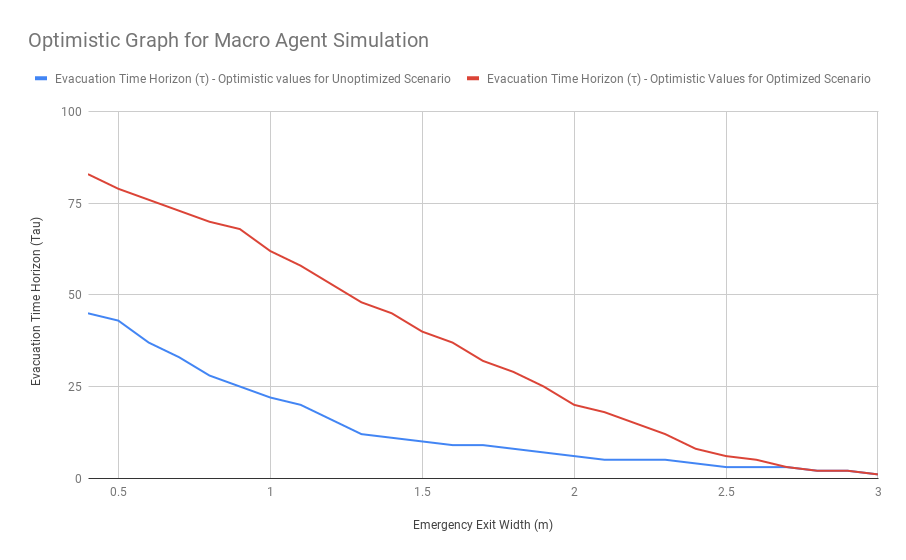
\includegraphics[scale=0.45]{simulation/Optimistic_Graph_for_Macro_Agent_Simulation.png}
  \caption{Optimistic Graph for Macro Agent Simulation}
  \label{Optimistic Graph for Macro Agent Simulation}
\end{figure}

\begin{figure}[H]
  \centering
  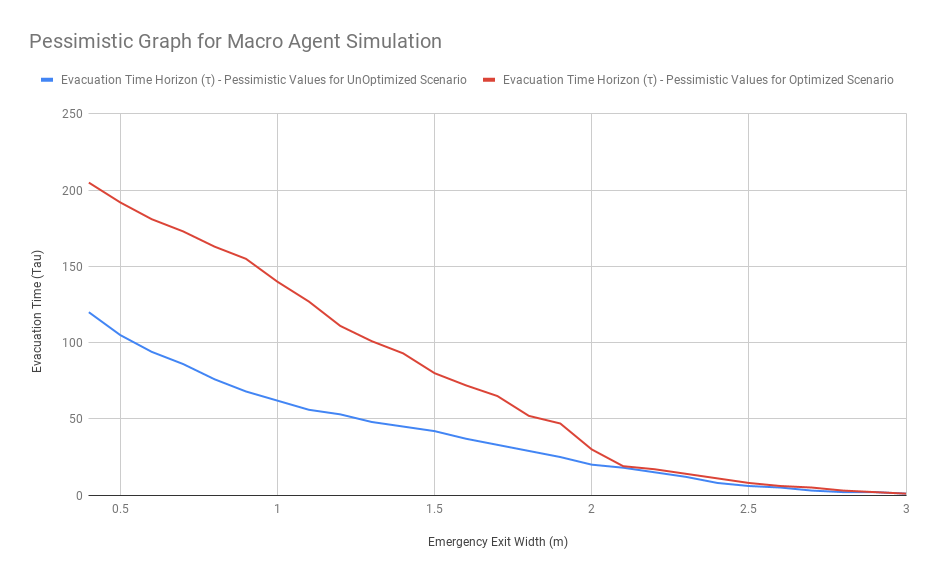
\includegraphics[scale=0.45]{simulation/Pessimistic_Graph_for_Macro_Agent_Simulation.png}
  \caption{Pessimistic Graph for Macro Agent Simulation}
  \label{Pessimistic Graph for Macro Agent Simulation}
\end{figure}

\begin{figure}[H]
  \centering
  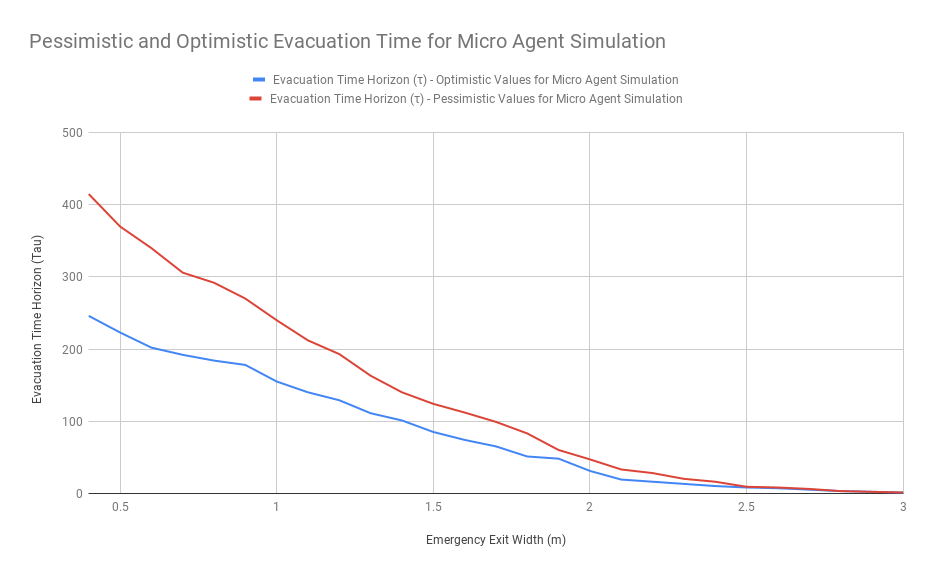
\includegraphics[scale=0.45]{simulation/Pessimistic_and_Optimistic_Evacuation_Time_for_Micro_Agent_Simulation.png}
  \caption{Pessimistic and Optimistic Evacuation Time for Micro Agent Simulation}
  \label{Pessimistic and Optimistic Evacuation Time for Micro Agent Simulation}
\end{figure}

\begin{figure}[H]
  \centering
  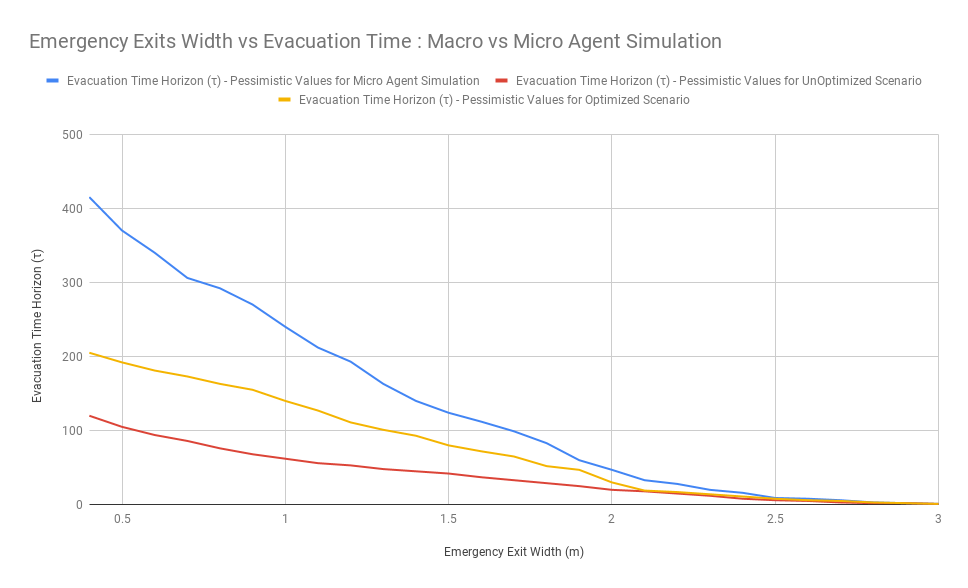
\includegraphics[scale=0.45]{simulation/summary.png}
  \caption{Emergency Exits Width vs Evacuation Time : Macro vs Micro Agent Simulation}
  \label{Emergency Exits Width vs Evacuation Time : Macro vs Micro Agent Simulation}
\end{figure}

From the above figures, it is made abundantly clear that the shorter the width of the exits, the more time it would take for the evacuees to evacuate during a disaster scenario. Though this seems like a trivial scenario to depict, it has some serious implications. The most important inference that can be made from the presented data is the derivation of how many people can effectively navigate through to an exit during a disaster scenario. The presented scenario compares the obtained statistical data to the reference figure 8 from \cite{ref5}.

It is also made clear that with more constraints and more realism, the statistical data shows that the congestion tends to increase as the evacuees tend to take longer and longer time to evacuate. Especially in the final scenario with the pessimistic values denoted for the micro model agent simulation, the evacuation time required to get all the agents to safety is exponential compared to the previous cases. The difference between pessimistic case and the optimal one is that in the optimistic case, only the shortest possible path towards the exit is considered. However, for the pessimistic case, all possible exit strategies are considered and hence the pessimistic case scenario should be considered whilst modeling a safe topology that caters for safe exit paths.

It should also be mentioned that the social distances in the micro agent simulations are set according to the UK fire safety regulations \cite{ref27} and the correponding guide given at \cite{ref28}. The guide specifies that the maximum allowed density is 0.3 square meters per person, 0.5 for public houses, 0.8 for exhibition spaces, 1.0 for dining and 2.0 for sports areas etc. From \cite{ref5}, who also follows the same regulations, 1.25 persons per square meter is considered. Hence for this scenario, the social distances constraint is set accordingly. The area capacity constraints that are set throughout all these experiments are set according to these regulation standards. In our case, since its clearly mentioned that not more 6 are allowed within an office space, each room cannot hold more than 6 people at a single time.

Figure \ref{Emergency Exits Width vs Evacuation Time : Macro vs Micro Agent Simulation} presents a summary of all the congestion scenarios. The pessimistic values that are obtained from the micro agent scenario shows the difference in the exponentiation graphs where the time taken for evacuation exponentially increases with a time complexity of $O(N^3)$ as the width of the exits are decreased.  

\subsection{Case 4: Shortest Path vs Ideal Path}
\label{sec: Case 4: Shortest Path vs Ideal Path}

This section presents the evacuation of agents and the time required based on the scenario of shortest path and the ideal paths. The shortest path in realistic scenario may not always be the shortest time path. Hence it is required to re-route the agents to a more optimal path, i.e. the ideal path in order to reach the exit points. In order to identify the ideal path, the algorithm traveses through all possible paths from the given agent location and then based on flow capacity and congestion ratio, it strategizes an ideal path for the agents to take whilst heading towards the safe zone. 

The ideal path formation depends on some factors which are given below:

\begin{itemize}
  \item Number of people in the group - this is used in calculation of the ideal path as the number of people in a group can be used to determine if other cluster of agents can form a congestion or not. It falls under congestion control and prediction.
  \item The movement speed of the group - this is used to calculate the ideal path by predicting if the group can reach a certain location or not to avoid congestion and cluster, if the group can access for instance an emergency service like elevators, emergency stairwells, exits etc.
  \item Area capacity - This is used to determine if the agent(s) are to be re-routed to another path.
  \item Door and cell flow dynamic- cell flow dynamic is used to determine if the stream of agents can be navigated through or not, to determine if a certain pathway is one way navigation only or not. The door flow capacity is used to determine the queuing and wait time as most congestions occur at key door and exit points. 
\end{itemize}

The above mentioned conditions are incorporated in this scenario in order to scan through all the possible paths and then determine an ideal path for the agents. Since walking speeds play an important role in determining routing path, it became a necessity to group people according to \textit{Energetic consequences of human sociality: walking speed choices among friendly dyads} by Wagnild et al. \cite{ref24}. According to Wagnild male agents walk at a faster pace when they are alone at an average speed of 1.53 $m/s$. They walk the fastest with a male companion at a speed of 1.60 $m/s$. The speed is subsequently lowered in the presence of a female agent to match her speed, which comes to around 1.44 $m/s$. Females walk even slower when accompanied with a female partner at a speed of 1.39 $m/s$. 

The mentioned walking speeds are done so in order to account for the expense of calories spent whilst walking. Men tend to reduce their speeds while walking with a female partner, female agents similarly increase their speeds and the compromized speed averaging at 1.44 $m/s$ is set upon. All the agents presented in the study are capable adults with no apparent health problems. 

However in order to make a realistic approach to simulation, all age groups should be considered. Hence for this case, 20\% of the total number of agents are considered agents with slower movement speeds, i.e., between 0.7 $m/s$ and 1.2 $m/s$. All the other agents are given a random speed between 1.2 and 1.6 $m/s$. The door flow capacity is set to not more than 5 for pessimistic cases as the same value has been used in \cite{ref5}, to remain coherent with the statistics. The upper limit, i.e. optimistic value is no more than 16 persons can pass through a 1 meter wide door during one time slot $\tau$. 

In order to model the exact movement speed of an agent within the PedSim environment, the total time required to move an agent across the entire breadth of the topology recorded and then subsequently divided by the total time taken in order to calculate the average speed that is taken by the agent to traverse 1 $m$ of the topology. This then can be used to set variable speeds according to aforementioned constraints and then the scenario is run within the environment of PedSim. The following graphs depict the pessimistic and the optimistic values that are obtained as a result of the simulations. However, for macro agent scenario, a movement speed based on the normal distribution across all agents is set.

The observational data from \cite{ref5} is used as a baseline reference in order to conduct the forthcoming simulations. For proper analysis and comparison, the initial number of agents present are taken as the same, i.e. $N = 1008$. The study is presented as follows:

\begin{figure}[H]
  \centering
  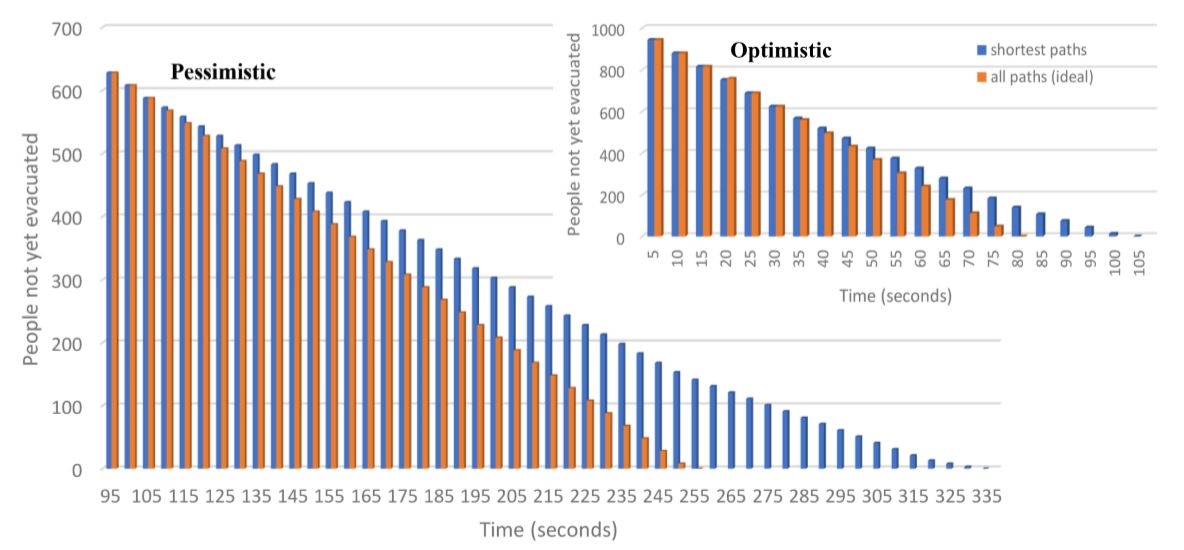
\includegraphics[scale=0.5]{simulation/ideal_evacuation_along_shortest_paths.JPG}
  \caption{Ideal Evacuation vs Shortest Path Evacuation Along Shortest Path for Macro Agents}
  \label{Ideal Evacuation vs Shortest Path Evacuation Along Shortest Path for Macro Agents}
\end{figure}

The above figure represents the number of people who can be evacuated within the given time frame for both pessimistic and optimistic cases, while simulating the whole scene for macro agent scenario. The pessimistic scenario runs for a total of 5 minutes and 35 seconds while the optimistic scenario runs for a total of 1 minute and 20 seconds. The figure below depict the cases for optimistic scenario that run on an macro agent model simulating an optimized scenario for path routing.

\begin{figure}[H]
  \centering
  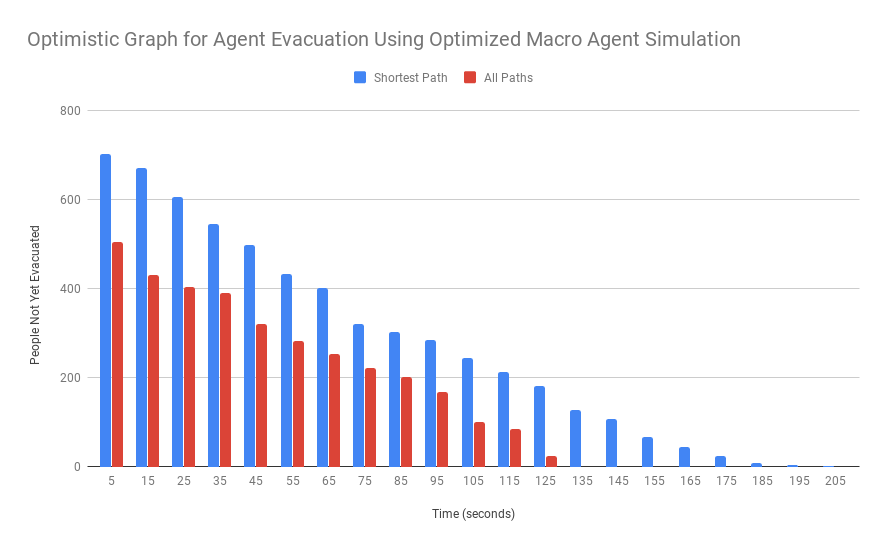
\includegraphics[scale=0.5]{simulation/Optimistic_Macro.png}
  \caption{Optimistic Graph for Agent Evacuation Using Optimized Macro Agent Simulation}
  \label{Optimistic Graph for Agent Evacuation Using Optimized Macro Agent Simulation}
\end{figure}

Compared to the previous figure \ref{Ideal Evacuation vs Shortest Path Evacuation Along Shortest Path for Macro Agents} depicting the optimistic scenario, its immediately evident that evacuation required is longer compared to and the number of agents that are not evacuated stays on for a longer period of time. This is with an increased capacity for the pathways since its the optimal scenario. The simulation takes a total of 3 minutes and 15 seconds in order to evacuate all people to safety. Some of the inferences made are as follows:

\begin{itemize}
  \item The interesting result to note is at the end tails of both the graphs. The graph from figure \ref{Ideal Evacuation vs Shortest Path Evacuation Along Shortest Path for Macro Agents} shows that the agents that follow the shortest paths tend to be evacuated last compared to the agents that follow the ideal path scenario based on the computation of all path.
  \item In the optimized macro agent case, we observe a similar trend where in the pattern of behavior as agents that follow either path strategy have similar evacuation times just like figure \ref{Ideal Evacuation vs Shortest Path Evacuation Along Shortest Path for Macro Agents}. 
  \item This is due to the fact that, in the results provided in \ref{Ideal Evacuation vs Shortest Path Evacuation Along Shortest Path for Macro Agents}, the agents flow plainly till the third of the total evacuation time and then the agents that follow the shortest path strategy start to experience congestion, while the agents that follow all paths strategy can evacuate quicker.
  \item A similar phenomenon is experienced in the presented optimized macro agent scenario as depicted in \ref{Optimistic Graph for Agent Evacuation Using Optimized Macro Agent Simulation} as the computation time required for both shortest path and ideal paths are the same for very low number of agents and hence for very low number of agents the evacuation time required is similar. However since the start number of agents are very high, the shortest path strategy experience congestion and hence takes more evacuation time.
  \item This however becomes very different for very large number of agents and as it can be seen from the graph \ref{Optimistic Graph for Agent Evacuation Using Optimized Macro Agent Simulation}, the curve becomes exponential ($O(N^2)$), for the shortest path strategy and increases steadily as the number of agents increase. The increase in number of agents cause higher congestion and hence the exponential increase in the evacuation time.
\end{itemize}

The next step is to compare the differences in scaling between the pessimistic case for  macro agent model simulated in an unoptimized scenario and the pessmisictic case for macro agent model running on the optimized constraints scenario. The prediction is that the rates of scaling will be very drastic as the pessimistic case reduces the flow capacity and also considers a few of the exits blocked. For the purposes of this experiment it was assumed that 2 out of 4 exits were blocked due to a static emergency like earthquake and hence the agents have to be re-routed to safety through the other exit points. This case is particularly interesting as congestions can be observed and how the agents tackle these congestions through predictive re-routing can be observed. 

The next figure \ref{Pessimistic Graph for Agent Evacuation Using Optimized Macro Agent Simulation} presents the aforementioned case.

\begin{figure}[H]
  \centering
  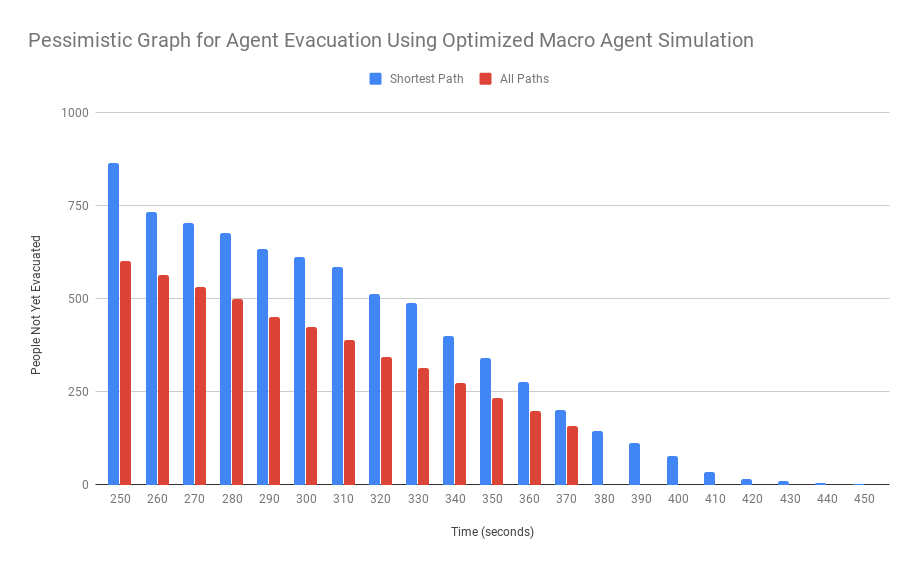
\includegraphics[scale=0.5]{simulation/Pessimistic_Macro.png}
  \caption{Pessimistic Graph for Agent Evacuation Using Optimized Macro Agent Simulation}
  \label{Pessimistic Graph for Agent Evacuation Using Optimized Macro Agent Simulation}
\end{figure}


The above represented graph typically confirms the previously described hypothesis in terms of scaling. As it can be observed quite clearly, the time required for the evacuation of agents in comparison to the figure \ref{Ideal Evacuation vs Shortest Path Evacuation Along Shortest Path for Macro Agents} is almost 1.5 times the time required for the evacuation for the same case presented.

The following are some inferences that are derived from the above graph:

\begin{itemize}
  \item Evidently the tail end of the graph for agents following the shortest path strategy raises exponentially ($O(N^2)$)
  \item The agents following the all paths strategy only increase linearly as the number of agents increase.
  \item The implications of these scaling differences are especially important as it can be further broken and analyzed as to which of the constraints cause this peak in scaling. Upon further investigation into the particular constraint causing the computation time difference, it is found that changing the values of area capacity and flow capacity makes most of the difference.
\end{itemize}

The next two cases present the optimistic and the pessimistic cases of the micro agent model scenario.

\begin{figure}[H]
  \centering
  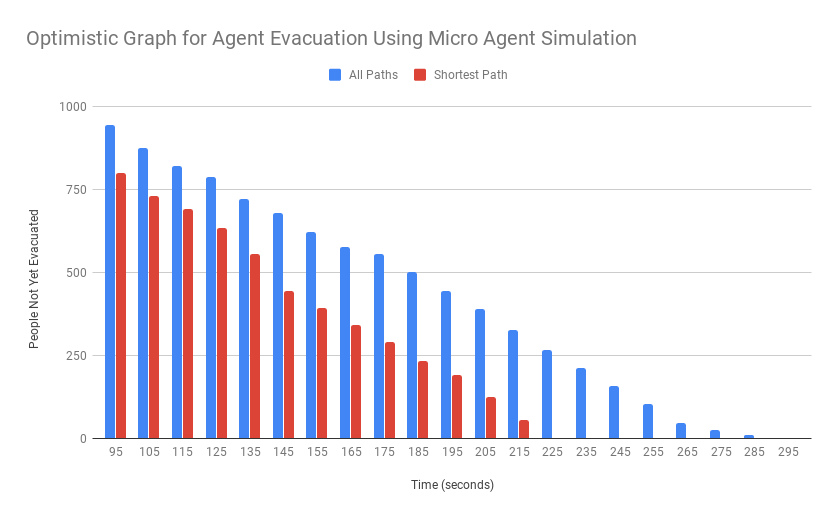
\includegraphics[scale=0.5]{simulation/Optimistic_Micro.png}
  \caption{Optimistic Case for Ideal Evacuation vs Shortest Path Evacuation Along Shortest Path for Micro Agents}
  \label{Optimistic Case for Ideal Evacuation vs Shortest Path Evacuation Along Shortest Path for Micro Agents}
\end{figure}

The figure given above depicts an interesting scenario compared to its counter part - the pessimistic case as presented in \ref{Ideal Evacuation vs Shortest Path Evacuation Along Shortest Path for Macro Agents}. Inferences from the given diagram will be presented below while discussing the following figure.

\begin{figure}[H]
  \centering
  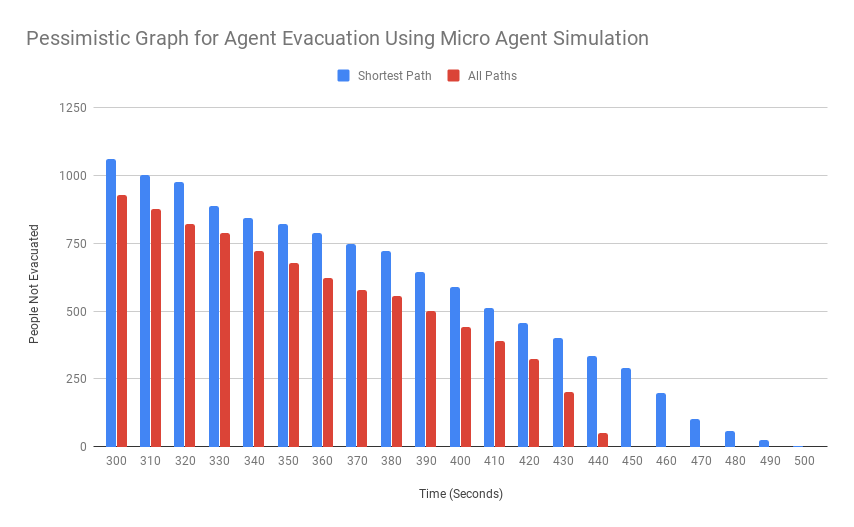
\includegraphics[scale=0.5]{simulation/Pessimistic_Micro.png}
  \caption{Pessimistic Case for Ideal Evacuation vs Shortest Path Evacuation Along Shortest Path for Micro Agents}
  \label{Pessimistic Case for Ideal Evacuation vs Shortest Path Evacuation Along Shortest Path for Micro Agents}
\end{figure}


The above two figures depict the interesting differences between the macro and micro agent simulation. As it can be observed from the figures \ref{Optimistic Case for Ideal Evacuation vs Shortest Path Evacuation Along Shortest Path for Micro Agents} and \ref{Pessimistic Case for Ideal Evacuation vs Shortest Path Evacuation Along Shortest Path for Micro Agents}, it takes longer than the macro agent model simulation in order to evacuate all the people to safety. The following inferences are presented in brief to compare and constrast between the obtained results:


\begin{itemize}
  \item It is important to note that the simulation performance changes that occur in \ref{Optimistic Case for Ideal Evacuation vs Shortest Path Evacuation Along Shortest Path for Micro Agents} when compared to the results obtained from the optimistic case presented in the figure \ref{Ideal Evacuation vs Shortest Path Evacuation Along Shortest Path for Macro Agents}.
  \item In an optimistic scenario, due to higher capacity and a higher degree of resulting congestion avoidance, the all paths strategy functions more optimally compared to its counter.
  \item This however becomes a more or less even for about 3 quarters of the evacuation time as is shown in figure \ref{Pessimistic Case for Ideal Evacuation vs Shortest Path Evacuation Along Shortest Path for Micro Agents}. The contrast in the evacuation time occurs due to the following reason:
    \begin{itemize}
      \item During a pessimistic scenario, it is assumed that 50\% of the total emergency exits are inaccessible due to a static emergency blockade. Hence as the numbers dwindle the time differnence between shortest paths and the all paths strategy becomes one and the same. Hence this causes the noticeable difference between the two results given above. 
    \end{itemize}
\end{itemize}

In summary it can drawn to a conclusion that the micro agent simulation with the all paths strategy takes the highest amount of time to evacuate, exhibiting a time complexity of $O(N^3)$. The macro agent model simulated with additional constraints takes a running time of $O(N^2)$.

% 
\chapter{Conclusion\label{ch:conclusion}}

From the presented scenario and cases, it is quite evidently evaluated that micro agent simulation, optimized with the applied realistic constraints presents the most realistic approach to evacuation compared to the other cases. Based on this objective presentation, we can design topologies and evacuation systems that are better suited to accommodate the required crowd of pedastrians. Through this thesis, it is also shown how adding even a small constraint to the simulation can severely alter the overall evacuation time of the agents. The nature of these constraints and how they affect the overall evacuation performance of the agents helps us to be better prepared in the likelihood of an actual disaster event.    

The present work employs a software architecture that helps improve and optimise the evacuation time which is very crucial in the case of an emergency. From the topology data obtained, it is pipelined into PedSim simulation environment. Once this data and the distribution of people is fed in to the system, the algorithm for evacuation provides a generic initial pathway to the agents and as time progresses, provides an alternate/optimal paths for various agents and suggest the paths suitable to each individual. This is achieved by dividing the floor plan first into blocks and subsequently into number of cells. The cells may have different orientations-horizontal and vertical. The paths are not allowed to cut through walls. The walls can be in any place even inside the rooms. Safe passage through the doors are then computed which connects to those to safe areas can then be computed. This modular nature of the algorithm makes it easy to scale the versions for future architecture and add more constraints by add-on modules. The simulation tool allows itself to upgraded to more generic pathing algorithm as well.  The following are the advantages that are due to the present simulation tool and the employed algorithm:

\begin{itemize}
\item All possible trajectories are computed.
\item The optimal paths to safe areas are selected from the same.
\item Regulates the flow as per the constraints to reduce congestions.
\item Erratic and random  motions are reduced.
\item Evacuation plan is made available to one and all.
\item Simulation is carried out in design time, although monitoring the status of evacuation is done in real time.
\item Can easily be integrated to IoT based framework.
\item Optimal evacuation procedure model can be evolved from the resulting simulations.
\end{itemize}

 % Conclusion
\section{Future Work}

This work can be extended to non-standard buildings with additional constraints in future. The internet of things (IoT) helps in locating the number of persons in each block and their location (cell numbers) which can then be dynamically fed in to the simulation tool for optimisation in real time. When such data can be obtained, the simulation can then be shifted from design time to a real time egress path evaluation. 


 
 % Future work

% \appendix % all chapters following will be labeled as appendices
% \chapter{Scenario Definition\label{ch:Scenario Definition}}

This section is used to provide a brief technical description of the implementation details that are involved whilst defining a scenario for the simulation of pedastrian agents within the PedSim environment. The library modules are written entirely in C++ whilst the topology description is described within a .xml file. The simulation tool parses the xml file and graphically projects the topology onto the simulation environment for visual reference.
The agent properties are also defined in the xml file such as their base speed, spawn location, total number of agents etc.

The section below provides an example of writing a topology description in the .xml file.

\section{Defining Topology}

The code snippet presented below depicts an example of defining the outline of the building, which was the topology used to run the simulations in. The dimensions of the building are strictly modeled according to the figure \ref{Coppito0 layout}. The dimensions have been scaled up to 5 times in order to suit the PedSim environment. A typical obstacle/wall description is defined as follows:
\\

\begin{lstlisting}[language=xml]
  <!-- Outer Walls -->
  
  <!-- TOP SIDE -->
  <obstacle x1="-120" y1="-90" x2="-7.5" y2="-90" />
  <obstacle x1="-7.5" y1="-90" x2="-7.5" y2="-60" />
  <obstacle x1="-7.5" y1="-60" x2="7.5" y2="-60" />
  <obstacle x1="7.5" y1="-60" x2="9.5" y2="-60" />
  <obstacle x1="17.5" y1="-60" x2="30" y2="-60" />
  <obstacle x1="30" y1="-60" x2="30" y2="-90" />
  <obstacle x1="30" y1="-90" x2="120" y2="-90" />

  <!-- RIGHT SIDE -->
  <obstacle x1="120" y1="-90" x2="120" y2="-15" />
  <obstacle x1="120" y1="-15" x2="105.5" y2="-15" />
  <obstacle x1="97.5" y1="-15" x2="97.5" y2="75" />

  <!-- BOTTOM SIDE -->
  <obstacle x1="97.5" y1="75" x2="7.5" y2="75" />
  <obstacle x1="7.5" y1="75" x2="4.5" y2="75" />
  <obstacle x1="-4.5" y1="75" x2="-7.5" y2="75" />
  <obstacle x1="-7.5" y1="75" x2="-97.5" y2="75" />
  <obstacle x1="-97.5" y1="75" x2="-97.5" y2="90" />
  <obstacle x1="-97.5" y1="90" x2="-135" y2="90" />


  <!-- LEFT SIDE -->
  <obstacle x1="-135" y1="90" x2="-135" y2="-30" />
  <obstacle x1="-135" y1="-30" x2="-112.5" y2="-30" />
  <obstacle x1="-120" y1="-38" x2="-120" y2="-90" />

\end{lstlisting}

From the above code snippet, the x and y pair points are given for drawing straight lines.
Partial and full agent pathing can be provided for the agents in order for them to start moving towards exit points during an emergency scenario.

\begin{lstlisting}[language=xml]

  <!-- waypoints are defined before agents  -->
  
  <waypoint id="w1" x="-75.0" y="-10" r="2" />
  <waypoint id="w2" x="-61" y="-3" r="2" />
  <waypoint id="w3" x="-50" y="-3" r="2" />
  <waypoint id="w4" x="-40" y="-3" r="2" />
  <waypoint id="w5" x="-30" y="-3" r="2" />
  <waypoint id="w6" x="-7.5" y="-3" r="2" />
  <waypoint id="w7" x="0" y="0" r="2" />
  <waypoint id="w8" x="0" y="30" r="2" />
  <waypoint id="w9" x="0" y="40" r="2" />
  <waypoint id="w10" x="0" y="50" r="2" />
  <waypoint id="w11" x="0" y="60" r="2" />
  <waypoint id="w12" x="0" y="70" r="2" />
  <waypoint id="w13" x="0" y="90" r="2" />

  \end{lstlisting}

The waypoint definition has coordianates x, y and radius r. The .xml file was written by referring the official documentation as provided in \cite{ref26}. Sample scenarios and tutorials regarding the same are also provided in the same documentation.

The final step in completing the scenario description is to include the agent properties. Given below is a sample agent definition in xml:

\begin{lstlisting}[language=xml]
  <agent x="30" y="-30" n="10" dx="50" dy="50">
  
  \end{lstlisting}

Where,
\begin{itemize}
\item $n$ is the number of agents.
\item $x$ and $y$ are the spawn location of the agents within the topography of the environment.
  \item dx and dy are used to determine the spread of the agents spawned. Agents are distributed evenly according to $x - dx$ and $x + dx$ and correspondingly along $y - dy$ and $y + dy$.
  \end{itemize}

Varying $n$ allows for defining the number of agents in a given group. This is particularly useful for the group simulation scenarios. In order to perform micro agent simulations, the $n$ is typically valued as 1. To summarize the agent definition, waypoints for the agents are defined in order to provide a more definitive pathing for the agents based on the spawn locations.

For a micro agent simulation, the agent definition will be as follows:
\\

\begin{lstlisting}[language=xml]
  
  <agent x="30" y="-30" n="1" dx="50" dy="60">
  <addwaypoint id="wu" />
  <addwaypoint id="wd" />
  <addwaypoint id="wz" />
  </agent> 
  <agent x="30" y="-30" n="1" dx="25" dy="30">
  <addwaypoint id="wu" />
  <addwaypoint id="wd" />
  <addwaypoint id="wz" />
  </agent> 
  <agent x="30" y="-30" n="1" dx="94" dy="100">
  <addwaypoint id="wu" />
  <addwaypoint id="wd" />
  <addwaypoint id="wz" />
  </agent> 
  <agent x="30" y="-30" n="1" dx="107" dy="112">
  <addwaypoint id="wu" />
  <addwaypoint id="wd" />
  <addwaypoint id="wz" />
  </agent>
    
\end{lstlisting}

Once the scenario to be modeled is described in the .xml file as given in the above code snippets, the file is then parsed by the PedSim library modules. Once the data is parsed from the .xml file, the agents are spawned according to the provided definitions and then PedSim proceeds to simulate the agents along the general waypoints as configured from the previous file.

The PedSim library modules are modified and extended in order to simulate the agents according to the algorithm present in \cite{ref5}. The technical details and description are provided in brief in the next section.
 

% \chapter{Printing and Binding\label{ch:printing}}

\section{Printing}

For the library copies of your dissertation, you must use archival quality printing and binding. This means acid-free paper, containing at least 25\% cotton fiber. Triangle Repocenter on Nassau Street in Princeton offers both 25\% cotton paper and 100\% cotton paper. Most people choose the 25\% cotton paper, and this is generally recommended by the binders. The 100\% copy paper is somewhat thicker and the extra expense is unnecessary. 

Triangle offers online submission of your printing and binding order at: \url{http://triangleprinceton.com/collegiatebinding/thesis/}. If you request binding from them, they will deliver the paper copies to Smith-Shattuck Bookbinding for you and allow you to pick up the completed copies at their store on Nassau Street. The whole process takes 2-3 business days, but check with them in advance during the busy thesis-printing season in April and May. 

Currently, your printed and bound dissertation copies can be single spaced. Only the electronic copy submitted to ProQuest must be double spaced. All copies must be printed single-sided, with specific margins. 

\section{Binding}

An archival-quality sewn binding is required for the library copies of your dissertation. Smith-Shattuck Bookbinding is highly recommended, and is used by most students. Triangle Repocenter will send your copies there for you, greatly simplifying the process, but you can call Smith-Shattuck with special requests. 

The ``library standard'' sewn binding is sufficient for the copies to be sent to Mudd Library. It uses a black buckram cloth cover, which is the most popular option. For extra copies for yourself and your family members, you can choose ``buckram roundback binding'', which adds decorative lines on the spine, and printing of the title and author on the front cover. For a small additional fee, you can include the Princeton University shield on the front cover and a ribbon bookmark. Leather covers are also available. See Smith-Shattuck's website for more details at: \url{http://www.thesisbookbinding.com/}. 


% Make the bibliography single spaced
\singlespacing
\bibliographystyle{plain}

% add the Bibliography to the Table of Contents
\cleardoublepage
\ifdefined\phantomsection
  \phantomsection  % makes hyperref recognize this section properly for pdf link
\else
\fi
\addcontentsline{toc}{chapter}{Bibliography}

% include your .bib file
\bibliography{thesis}

\end{document}

